%  article.tex (Version 3.3, released 19 January 2008)
%  Article to demonstrate format for SPIE Proceedings
%  Special instructions are included in this file after the
%  symbol %>>>>
%  Numerous commands are commented out, but included to show how
%  to effect various options, e.g., to print page numbers, etc.
%  This LaTeX source file is composed for LaTeX2e.

%  The following commands have been added in the SPIE class 
%  file (spie.cls) and will not be understood in other classes:
%  \supit{}, \authorinfo{}, \skiplinehalf, \keywords{}
%  The bibliography style file is called spiebib.bst, 
%  which replaces the standard style unstr.bst.  

\documentclass[]{spie}  %>>> use for US letter paper
%%\documentclass[a4paper]{spie}  %>>> use this instead for A4 paper
%%\documentclass[nocompress]{spie}  %>>> to avoid compression of citations
%% \addtolength{\voffset}{9mm}   %>>> moves text field down
%% \renewcommand{\baselinestretch}{1.65}   %>>> 1.65 for double spacing, 1.25 for 1.5 spacing 
%  The following command loads a graphics package to include images 
%  in the document. It may be necessary to specify a DVI driver option,
%  e.g., [dvips], but that may be inappropriate for some LaTeX 
%  installations. 
\usepackage{graphicx}
\usepackage{subfig}
\usepackage{amsmath}
\usepackage{amssymb}
\usepackage{hyperref}
\usepackage{float}
\title{Texture mapping 3D planar models of indoor environments with noisy camera poses} 

%>>>> The author is responsible for formatting the 
%  author list and their institutions.  Use  \skiplinehalf 
%  to separate author list from addresses and between each address.
%  The correspondence between each author and his/her address
%  can be indicated with a superscript in italics, 
%  which is easily obtained with \supit{}.

\author{Peter Cheng, Michael Anderson, Stewart He, Avideh Zakhor
\skiplinehalf
University of California, Berkeley\\
}

 

%%%%%%%%%%%%%%%%%%%%%%%%%%%%%%%%%%%%%%%%%%%%%%%%%%%%%%%%%%%%% 
%>>>> uncomment following for page numbers
% \pagestyle{plain}    
%>>>> uncomment following to start page numbering at 301 
%\setcounter{page}{301} 
 
\begin{document}
\maketitle

%%%%%%%%%%%%%%%%%%%%%%%%%%%%%%%%%%%%%%%%%%%%%%%%%%%%%%%%%%%%% 
\begin{abstract}
  Automated 3D modeling of building interiors is used in applications
  such as virtual reality and environment mapping. Texturing these
  models allows for photo-realistic visualizations of the data
  collected by such modeling systems. While data acquisition times for mobile mapping systems are considerably shorter than for static ones, their recovered camera poses often suffer from inaccuracies, resulting in visible discontinuities when successive images
  are projected onto a surface for texturing. Existing methods to
  stitch images together are often computationally expensive and work
  independently of pose estimates and geometry data. 

The approach in this paper minimizes complexity by refining camera poses in 2D, which works well given our high amount of images and minimal 3D pose errors. We also align images to geometry as well as to each other, which produces visually consistent textures even in the presence of inaccurate surface geometry. We also present two different methods for selecting and compositing images into a single texture, depending on the geometry of surfaces being textured. The effectiveness of our method is demonstrated on a number of different indoor environments.


By
  intelligently selecting images for texturing, we develop an
  efficient method to adjust camera poses in 2D, using linear features
  to match images to geometry, and point features to match images
  together. This is followed by two different methods to composite
  images together, based on the geometry of surfaces being
  textured. The effectiveness of our method is demonstrated on a
  number of different indoor environments.
\end{abstract}

% >>>> Include a list of keywords after the abstract

\keywords{Texture Mapping, Reconstruction, Image Stitching, Mosaicing}

%%%%%%%%%%%%%%%%%%%%%%%%%%%%%%%%%%%%%%%%%%%%%%%%%%%%%%%%%%%%%
\section{Introduction}
\label{sec:introduction} % \label{} allows reference to this section
Three-dimensional modeling of indoor environments has a variety of
applications in fields such as architecture, conservation, and
simulation. Applying accurate textures to these models is important to
add context to digital visualizations, and allows for image-based
analysis of environments. In this paper, we perform data acquisition
with a backpack-mounted system carried by an ambulatory human
\cite{liu2010indoor}. This backpack system contains 2 fisheye cameras
as well as laser scanners and inertial measurement units,
used to solve the simultaneous localization and mapping (SLAM)
problem, which produces backpack (and therefore camera) poses over
time as well as a point cloud representing the surrounding environment
\cite{chen2010indoor, liu2010indoor, kua2012loopclosure}. SHOW PICTURE OF BACKPACK. For
environment geometry, we work with models obtained by fitting
low-resolution planar surfaces to these point clouds
\cite{sanchez2012point}.

While a human-carried system provides advantages over more common
wheeled systems in terms of agility and portability, it often leads to
relatively high localization error even after applying sophisticated
localization techniques \cite{liu2010indoor}. Furthermore, our model
geometry usually contains some error as well, and is often tuned to
ignore low-resolution features, such as small walls, furniture, and
other minor non-planar features commonly found in indoor
environments. As a result, methods for texture mapping that rely on
accurate camera poses and projection surfaces generally produce poor
results, while more sophisticated methods to accurately align images
in 3D lead to high runtime on our typically very large datasets. In
contrast, we present a method, which given a high number of images,
searches for a subset of them that can be successfully aligned with 2D
adjustments alone.

The remainder of the paper is organized as follows. Section
\ref{sec:simpleTextureMapping} explains how images are projected onto
our geometry and explains a simple approach towards selecting images
for texturing. Section \ref{sec:existingApproaches} covers existing
approaches to image stitching, and their performance on our
datasets. Section \ref{sec:2dAlignment} contains our approach towards
efficient 2D image alignment, followed by Section
\ref{sec:imageCompositing}, which describes our two methods of
compositing images. Section \ref{sec:resultsAndConclusions} contains
results and conclusions.

%%%%%%%%%%%%%%%%%%%%%%%%%%%%%%%%%%%%%%%%%%%%%%%%%%%%%%%%%%%%%




\section{Simple Texture Mapping}
\label{sec:simpleTextureMapping}

The geometry of the texture mapping process for a planar surface is
shown in Figure \ref{fig:projection}.  We are provided with a set of
$M$ images to texture a target plane, where each image has a camera
matrix $P_i$ for $i=1..M$, which translates a 3D point in the world
coordinate system to a 2D point or pixel in image $i$'s coordinates. A
camera matrix $P_i$ is composed of the camera's intrinsic parameters,
containing focal length and image center, as well as extrinsic
parameters which specify the rotation and translation of the camera's
position in 3D world coordinates at the time that image $i$ is
taken. These extrinsic parameters are determined by the backpack
hardware and localization algorithms \cite{chen2010indoor,
  liu2010indoor, kua2012loopclosure} and are substantially noisy.

Because our backpack system takes photos at a rate of 5 Hz, hundreds
of images are available for texturing each surface in our model. Our
goal in designing a texture mapping process is to decide which of
these images should be used, and where their contents should map onto
the final texture, in order to minimize any visual discontinuities or
seams that would suggest that the plane's texture is not composed of a
single continuous image.

\begin{figure}
  \begin{minipage}[b]{0.45\linewidth}
    \centering
    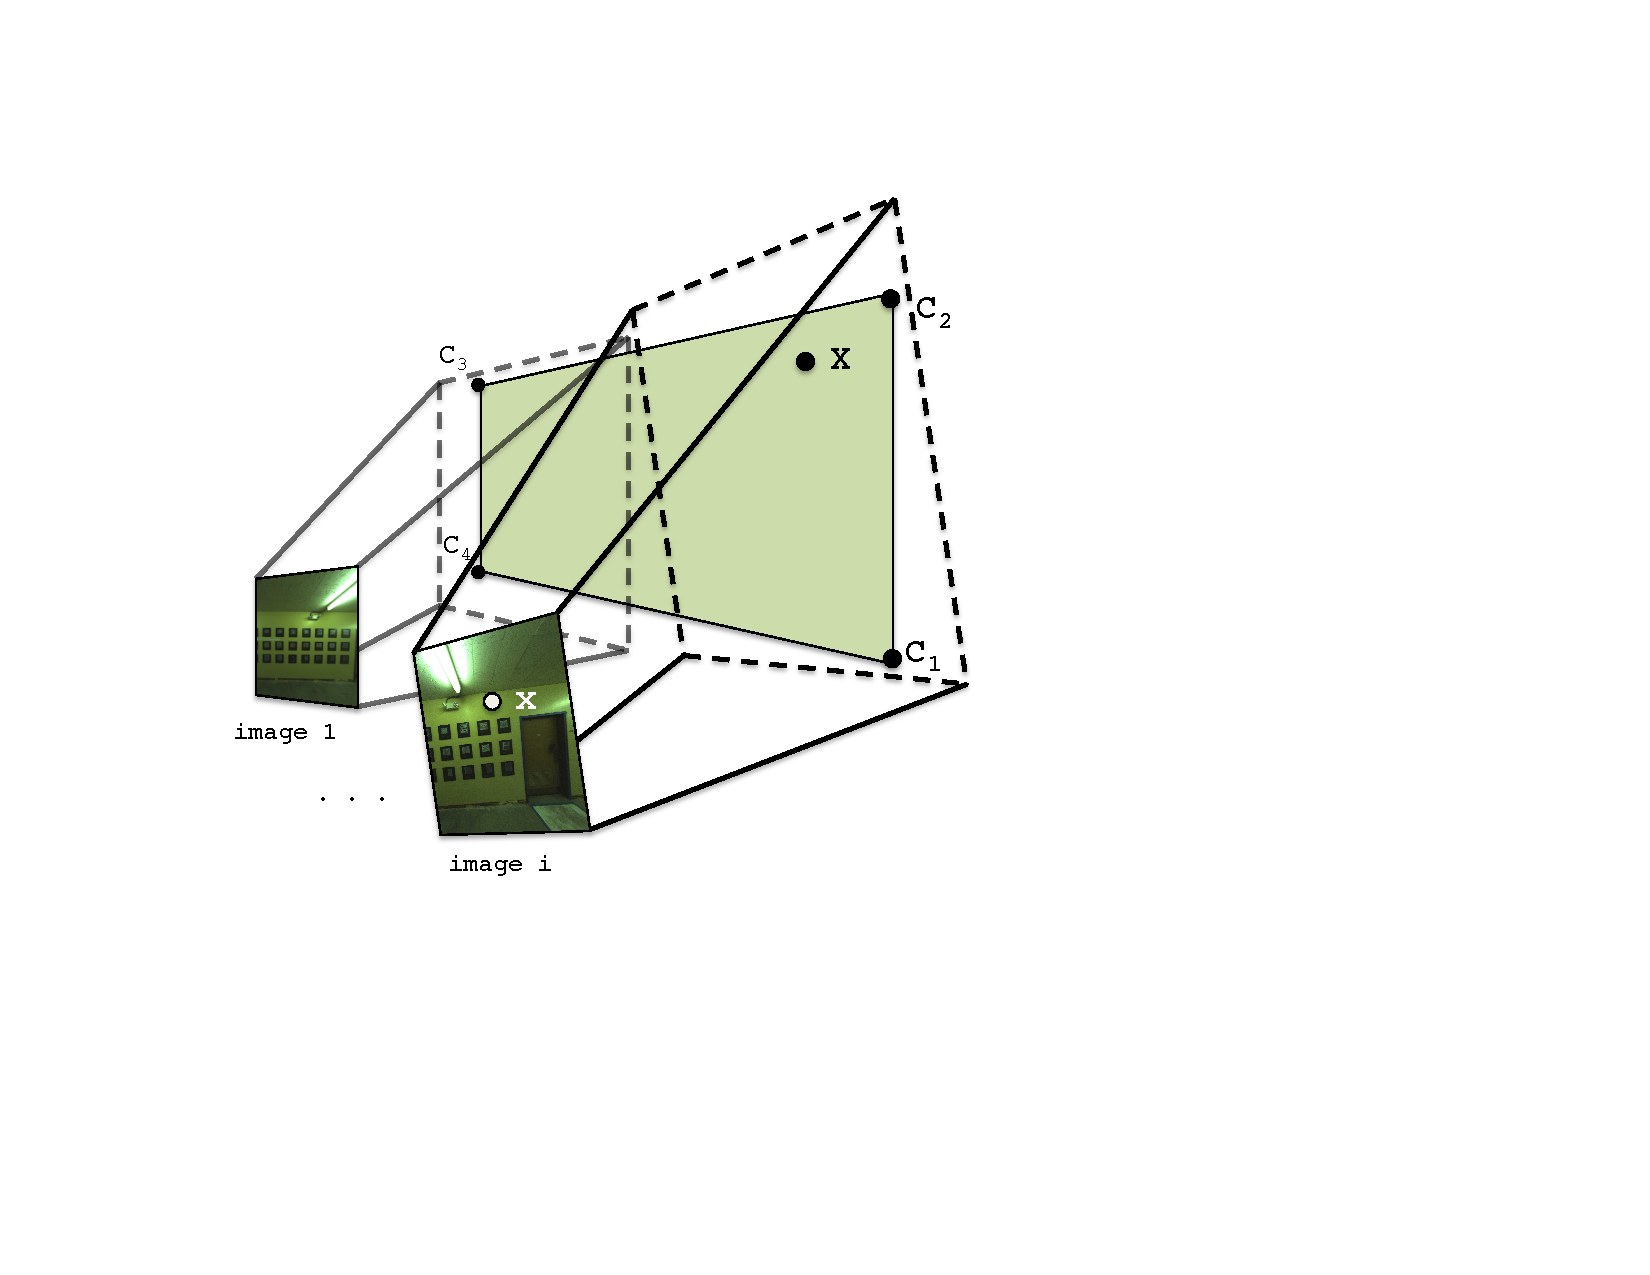
\includegraphics[height=1.8in]{Projection.pdf}
    \caption{Surfaces to be textured are specified in 3D space by
      corners $C_i$. Images are related to each surface through the
      camera matrices $P_{1..m}$. }
    \label{fig:projection}
  \end{minipage}
  \hspace{0.5cm}
  \begin{minipage}[b]{0.45\linewidth}
    \centering
    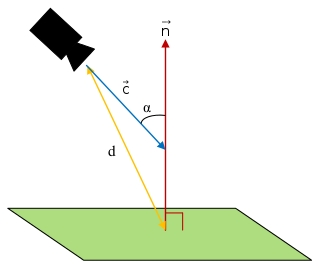
\includegraphics[height=1.8in]{scoringFunction.jpg}
    \caption{We minimize camera angle $\alpha$ and distance $d$ by
      maximizing the scoring function $\frac{1}{d} (-1 \cdot \vec{c})
      \cdot \vec{n}$}
    \label{fig:scoringFunction}
  \end{minipage}
\end{figure}


\subsection{Tile-based Texture Mapping}
\label{sec:tileBasedMapping}
Ignoring the fact that the camera matrices $P_{1..M}$ are inaccurate,
a simple texturing approach can be performed by discretizing the
target plane into small square tiles, and choosing an image to texture
each tile directly.

We choose to work with rectangular units to ensure that borders
between any two distinct images in the final texture are either
horizontal or vertical. Since most strong environmental features
inside buildings are horizontal or vertical, any visible seams in our
texture will intersect them minimally and be less noticeable.

In order to select an image for texturing a tile $t$, we first gather
a list of candidate images that contain all four of its corners, which
we can quickly check by projecting $t$ into each image using the $P_i$
camera matrices. Furthermore, each candidate image must have been
taken at a time when its camera had a clear line-of-sight to $t$,
which can be calculated using standard ray-polygon intersection tests
between the camera location, $t$, and every other plane
\cite{rayintersection}.

Once we have a list of candidate images for $t$, we define a scoring
function in order to objectively select the best image for texturing
$t$. Since resolution decreases and camera pose errors become more
extreme over distance, we wish to minimize the distance between
cameras and the surfaces they texture. Additionally, we desire images
that are projected perpendicularly onto the plane, maximizing the
resolution and amount of useful texture available in their
projections, as well as minimizing any parallax effects due to
real-world geometry not accurately represented by our digital
model. In other words, we wish to minimize the angle between the
tile's normal vector and the camera axis for images selected for
texturing that tile. These two criteria can be met by maximizing the
function $\frac{1}{d} (-1 \cdot \vec{c}) \cdot \vec{n}$ as shown in
Figure \ref{fig:scoringFunction}. Specifically, $d$ is the distance
between the centers of a camera and a tile, and $\vec{n}$ and
$\vec{c}$ are the directions of the plane's normal and the camera axis
respectively.


As Figure \ref{fig:compareAll}(a) demonstrates, there are many image
boundaries with abrupt discontinuities between tiles, due to
significant misalignment between images, though most of it appears to
be reconcilable using 2D transforms. Given our high number of input
images, a better image selection procedure will further improve
results, as described in Section \ref{sec:imageCompositing}, but a
more significant and reliable improvement can be found through first
improving the alignment of our images.

\begin{figure}[H]
  \centering \subfloat[][]{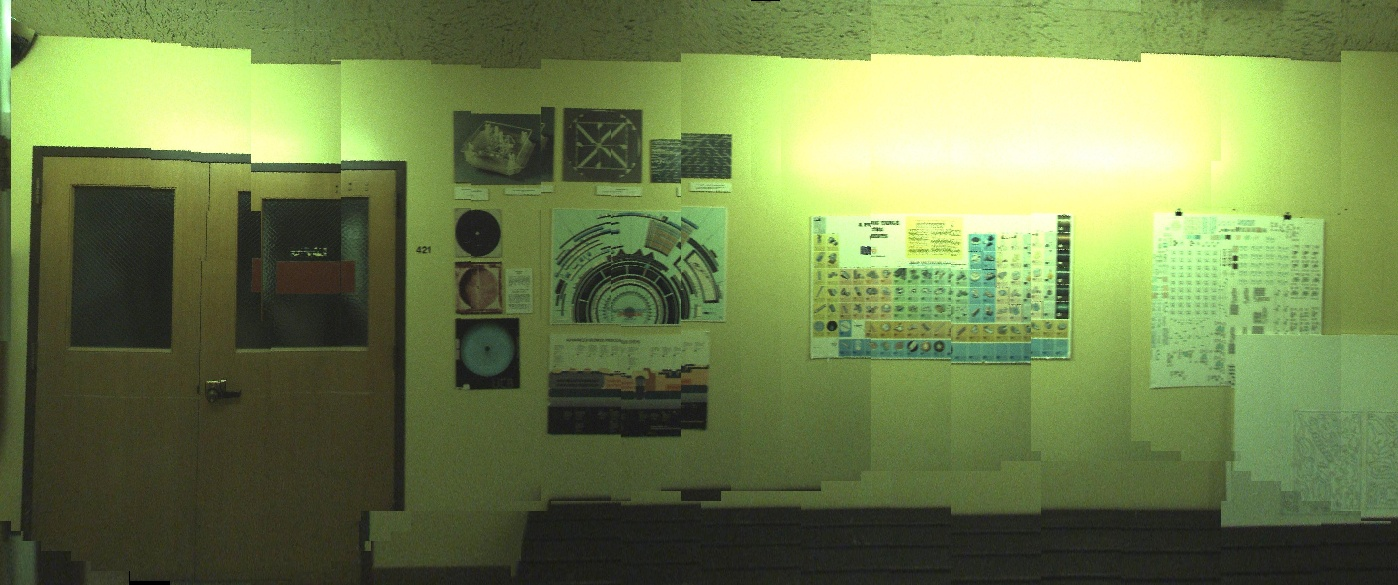
\includegraphics[width=3.4in,
    height=1.2in]{wall2_naive.jpg}}
  \subfloat[][]{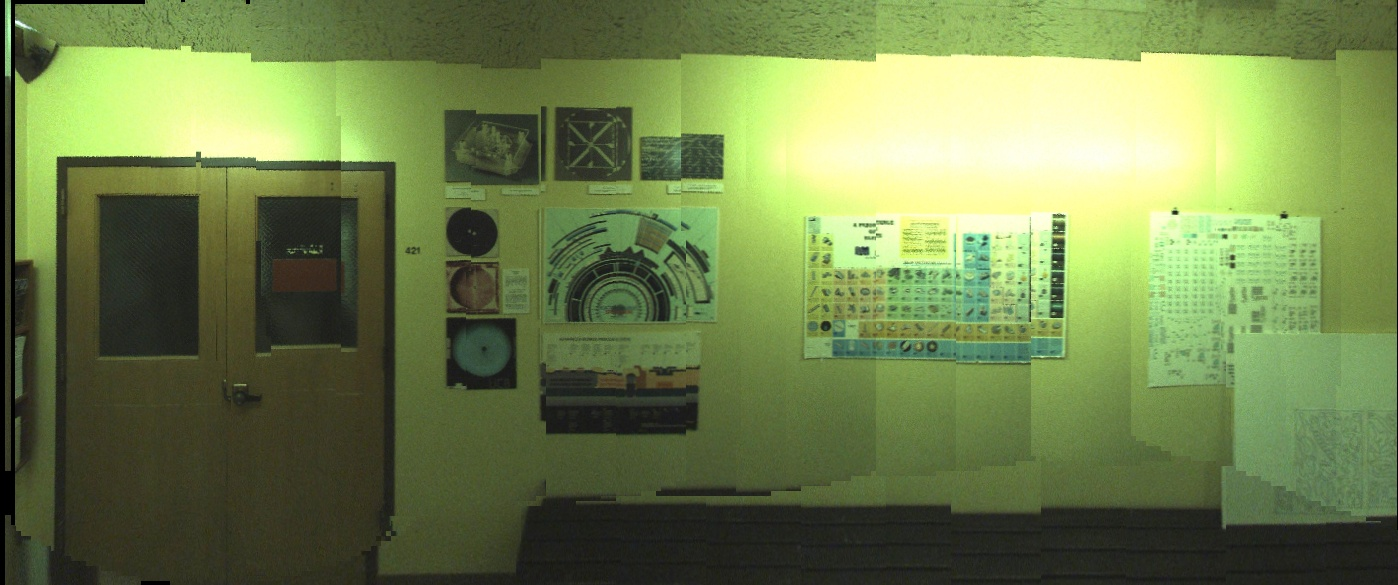
\includegraphics[width=3.4in,
    height=1.2in]{wall2_naive_shift.jpg}}

  \centering \subfloat[][]{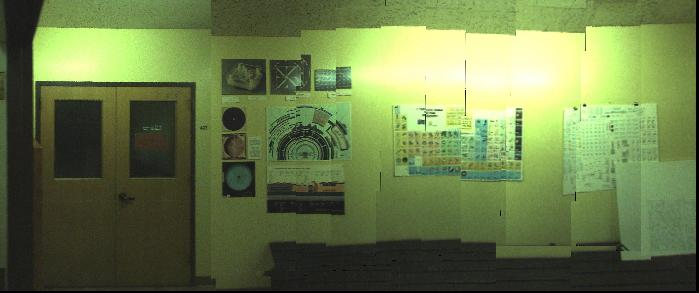
\includegraphics[width=3.4in,
    height=1.2in]{wall2_cache_shift.jpg}}
  \subfloat[][]{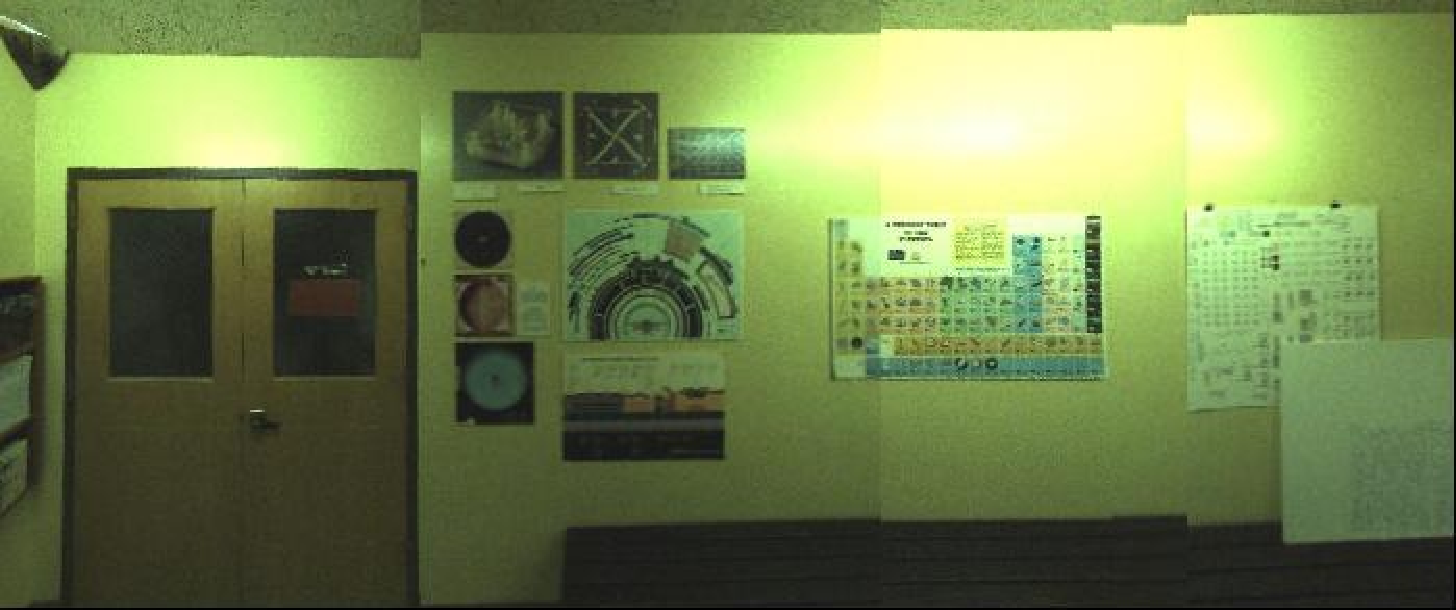
\includegraphics[width=3.4in,
    height=1.2in]{wall2_shortest_shift.pdf}}

  \centering \subfloat[][]{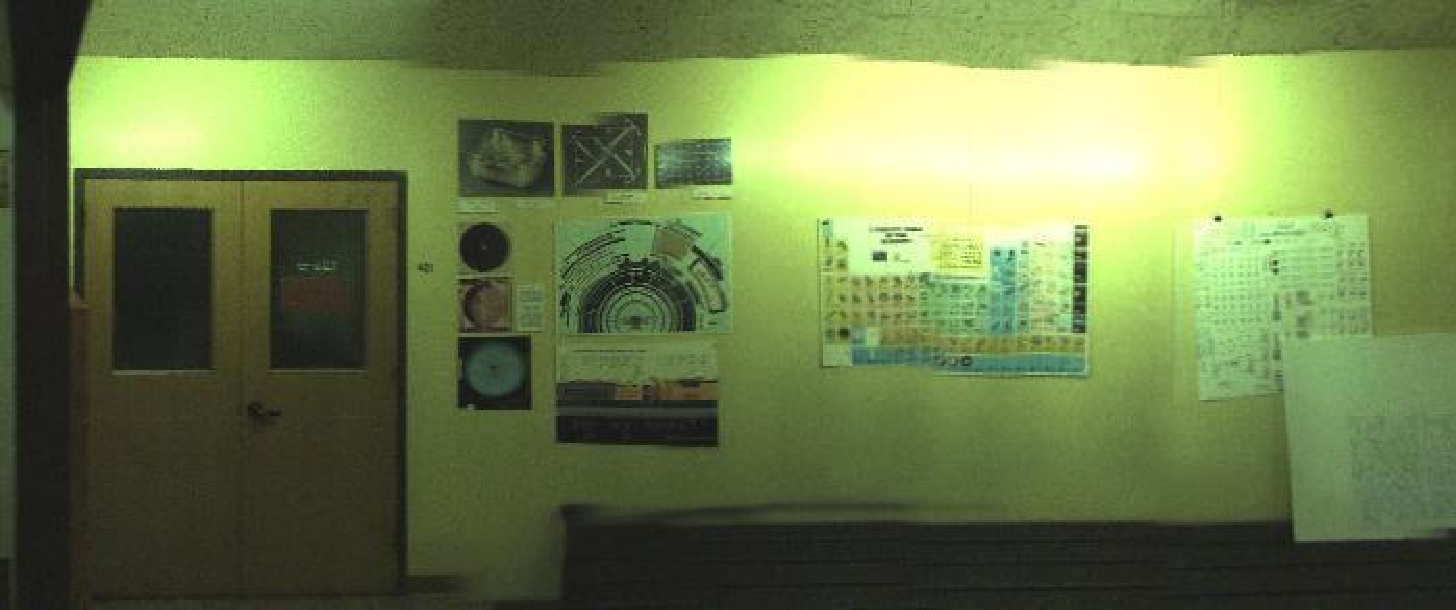
\includegraphics[width=3.4in,
    height=1.2in]{wall2_cache_shift_blend.pdf}}
  \subfloat[][]{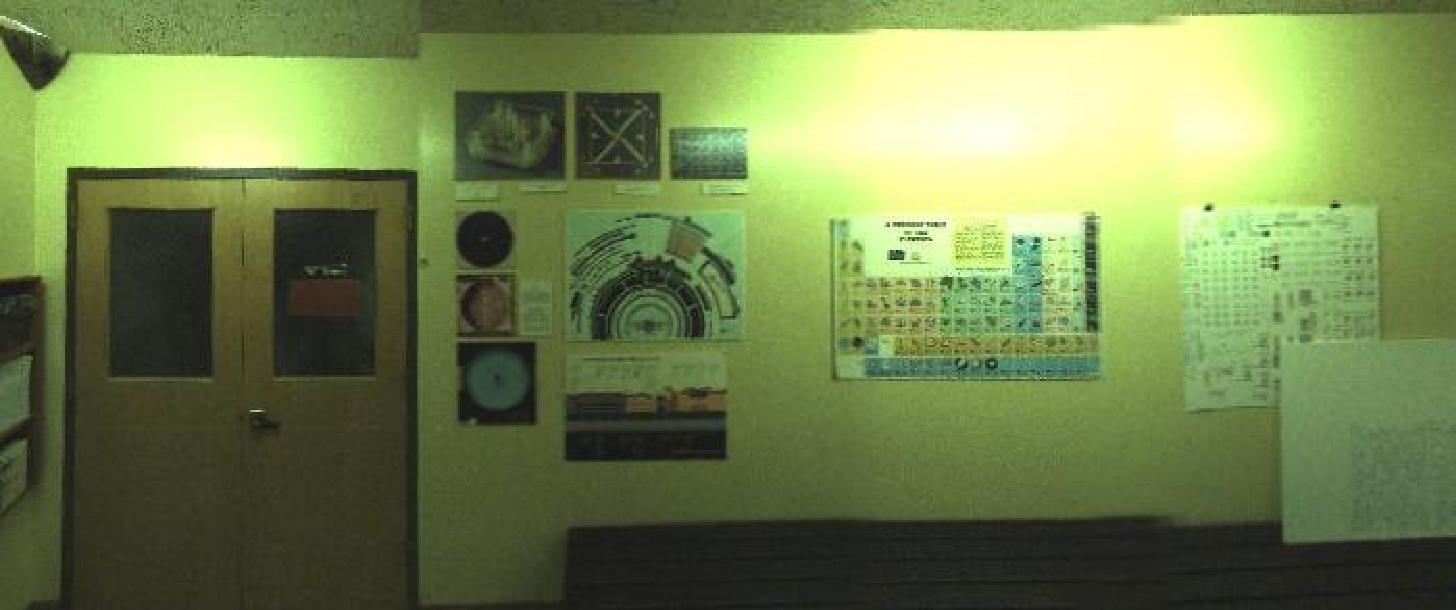
\includegraphics[width=3.4in,
    height=1.2in]{wall2_shortest_shift_blend.pdf}}

  \centering \subfloat[][]{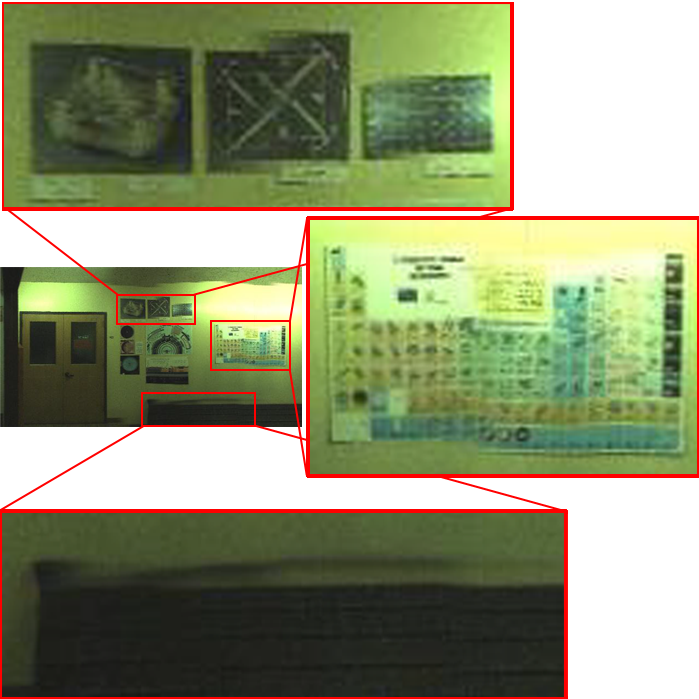
\includegraphics[width=3.4in,
    height=3.4in]{wall2_cache_comparison.png}}
  \subfloat[][]{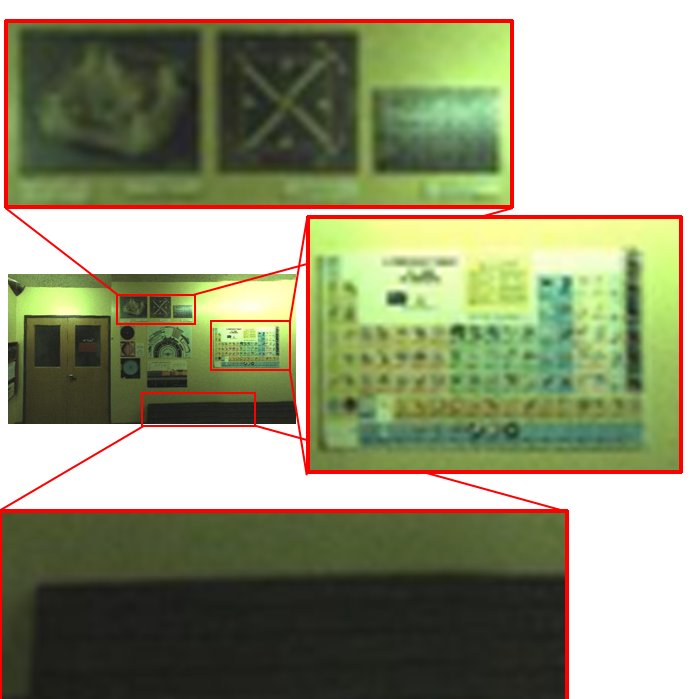
\includegraphics[width=3.4in,
    height=3.4in]{wall2_shortest_comparison.png}}

  \caption{(a): Tile-based texturing. (b): Tile-based texturing after
    image alignment. (c): Tile-based texturing after image alignment
    with caching. (d): Shortest path texturing after image
    alignment). (e,f): Blending applied to (c) and (d). (g,h): Zoomed
    in views of discontinuities in (e) vs. in (f).}
  \label{fig:compareAll}
\end{figure}


\section{Existing Approaches to Image Alignment}
\label{sec:existingApproaches}
Stitching together multiple images to produce a larger, seamless image
is a commonly performed task, with many successful approaches over the
past years. Generally, parts of images are matched to each other,
usually through direct comparisons or feature detection and
matching. Images are then transformed to maximize matches, often by
calculating homographies between pairs of images, or by iteratively
adjusting camera poses in 1 to 6 degrees of freedom.

Feature matching has a number of advantages over direct matching that
make it more suitable for our often non-planar data, and rotational
differences \cite{szeliski2006image}. Feature matching however, works
best when multiple unique visual references exist in the environment
that can be detected in multiple images. In contrast, our indoor
environments have a high prevalence of bare surfaces, as well as
repeating textures, such as similar windows, doors, and wall-mounted
decorations, that cause difficulty in disambiguating features. This
lack of reliable reference points often results in errors when
matching images together.

Additionally, our datasets often contain long chains of images, which
can lead to large overall error when images are matched together. For
example, a slight error in image correspondences in the middle of a
chain could lead to high global error at one or both ends of the
chain.

\begin{figure}
  \centering
  \subfloat[][]{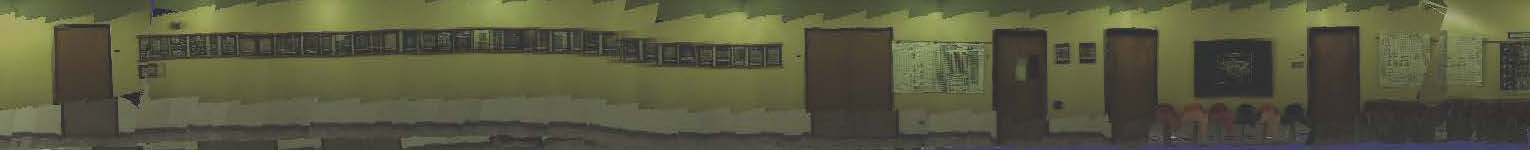
\includegraphics[width=6in]{graphApproach.jpg}}

  \centering
  \subfloat[][]{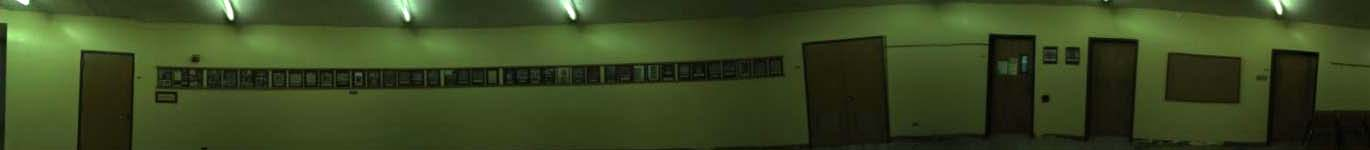
\includegraphics[width=6in]{autostitchResult.jpg}}

  \centering \subfloat[][]{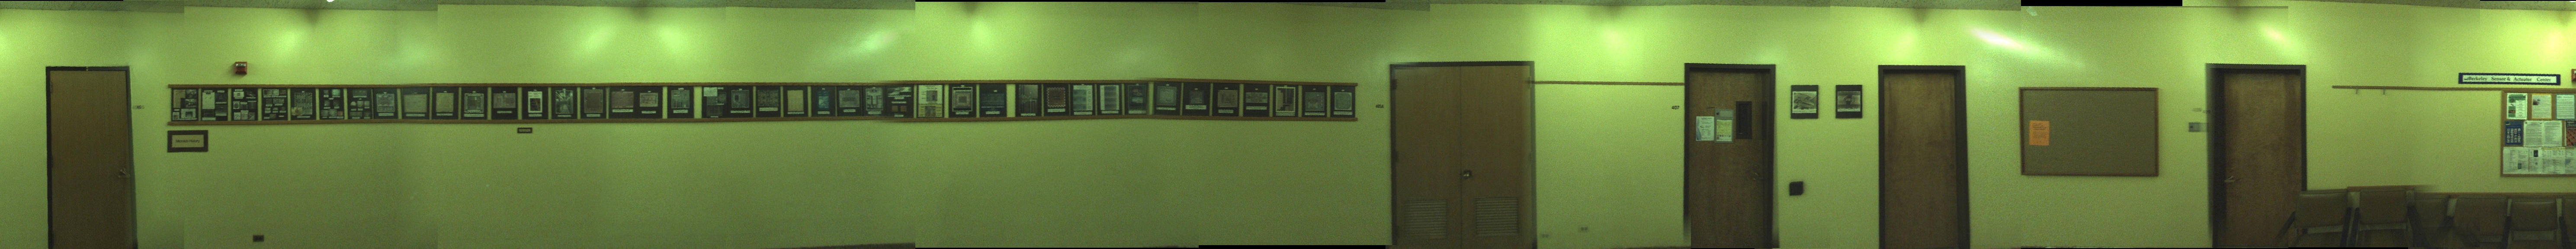
\includegraphics[width=6in]{finalLong.jpg}}

  \caption{Texture alignment via (a) the graph-based localization
    refinement algorithm, (b) the AutoStitch software package, and (c)
    our method.}
  \label{fig:mosaic3D}
\end{figure}


Past work with our data acquisition backpack integrated image
stitching with an iterative localization algorithm, and performed
homography-based camera pose refinement \cite{liu2010indoor}. When run
on long chains of images, especially where features are sparse, it
produces distorted textures, as seen in Figure \ref{fig:mosaic3D}(a),
due to the problems described above. This approach is also not
closed-form, and its iterative camera adjustment process over our
large datasets led to prohibitively long computation time.

The AutoStitch software package performs homography-based alignment as
well, with additional provisions that attempt to reduce drift and
increase efficiency \cite{panorama2d, autostitch}. Though AutoStitch
also performs well in areas with dense features, it can not handle
areas without features, and has trouble aligning wall sections with
even short segments of bare texture. The example in Figure
\ref{fig:mosaic3D}(b) was generated after manual tuning, and areas
with fewer visual features or repeating texture patterns simply failed
outright with AutoStitch.

More importantly, neither approach 



\section{2d Image Alignment}
\label{sec:2dAlignment}

In this section, we describe our method of efficient and robust image
alignment. Though state-of-the-art techniques towards image stitching
work in 3D, we elect to perform image alignments entirely in
2D. Besides the benefits of reduced complexity, we have found 2D
alignment to work well for two main reasons. First, because we have
such a large number of images to choose from, the compositing
approaches in Section \ref{sec:imageCompositing} are able to select a
subset of images that align well, given only 2D alignments. Second,
the nature of our input data is such that localization error chiefly
occurs in two dimensions, in the same plane as the surface being
projected onto. Our data acquisition system contains cameras facing to
the sides of the operator. The operator makes efforts to walk parallel
to walls, and the localization and model-generation algorithms that
provide our input conform the operator's path to be straight and
parallel to detected surfaces \cite{kua2012loopclosure,
  sanchez2012point}. Since the operator also walks in a manner to keep
the backpack balanced, errors in roll and yaw are minimal. Thus, our
highest errors stem from uncertainty in the operator's pitch,
equivalent to rotation around the camera axes, as well as location
along surfaces. These equate to 2D rotation and translation in a
surface's plane.

Our 2D alignment procedure consists of three parts. First, all images
are projected onto the surface and lines within these projections are
detected. These lines are then rotated and shifted to match
geometry-based lines comprising the surface's boundary and
intersection with other surfaces. Second, occlusion checks are
performed to remove invalid parts of each image for the target
surface. These two steps are image-independent and performed in
parallel. Third, we detect SIFT feature matches between pairs of
images and solve a weighted linear least squares problem in 2D to
maximize matches.

\subsection{Geometry-based Alignment}
\label{sec:geometryAlignment}
After computing each image's projection onto the target surface, as
described in Section \ref{sec:simpleTextureMapping}, we detect line
segments in the image projections using Hough transforms, as shown in
Figure \ref{fig:geometryAlignment}(a). Experience and intuition show
that walls in indoor environments often contain linear features that
are either horizontal or vertical, corresponding to doors, windows,
posters, etc. Thus, when texturing walls, we rotate images in 2D such
that dominant lines are made to be horizontal or vertical. This can be
further generalized by instead orienting lines to be parallel or
perpendicular with a surface's boundaries, which makes it applicable
to ceilings and floors, where inner walls and interior features tend
to be parallel or perpendicular to outer walls.

\begin{figure}
  \centering
  \subfloat[][]{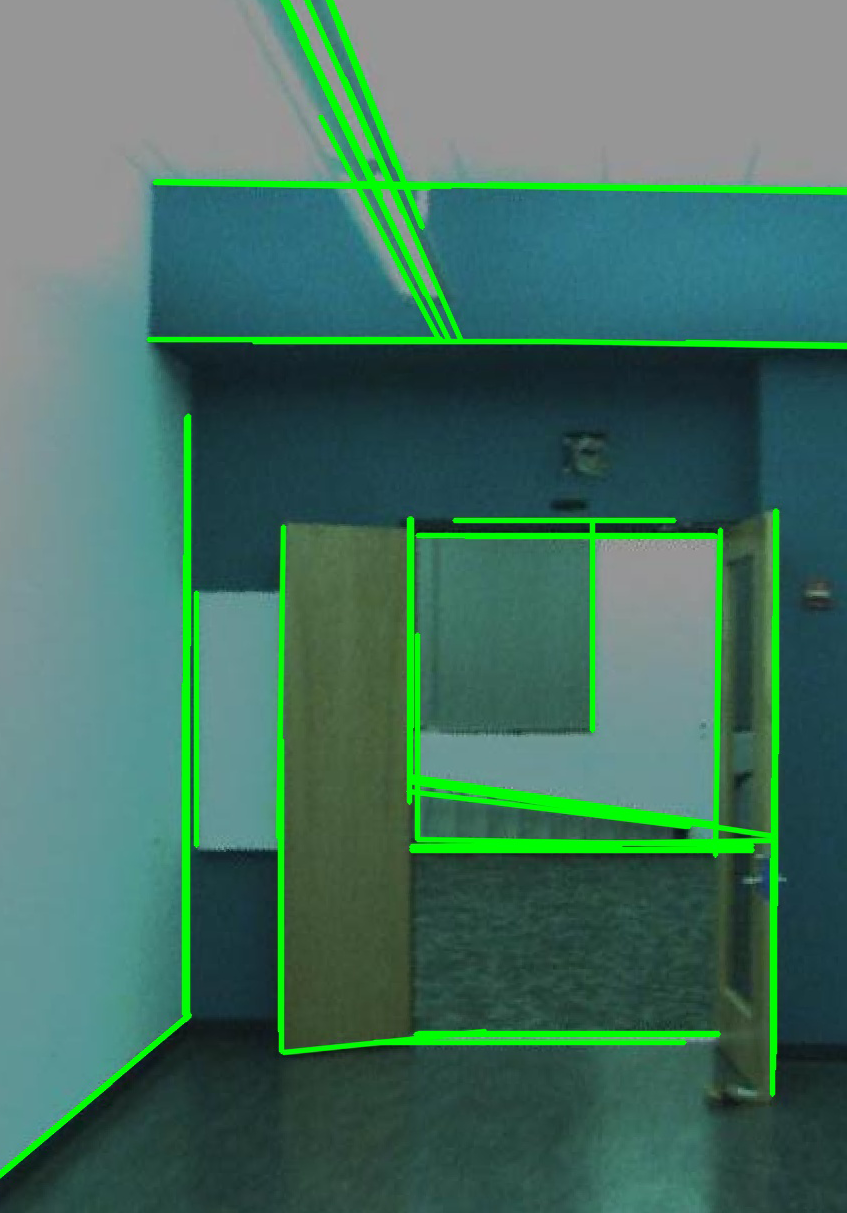
\includegraphics[height=3in]{detectedLines.png}}
  \hspace{0.4 cm} \subfloat[][]{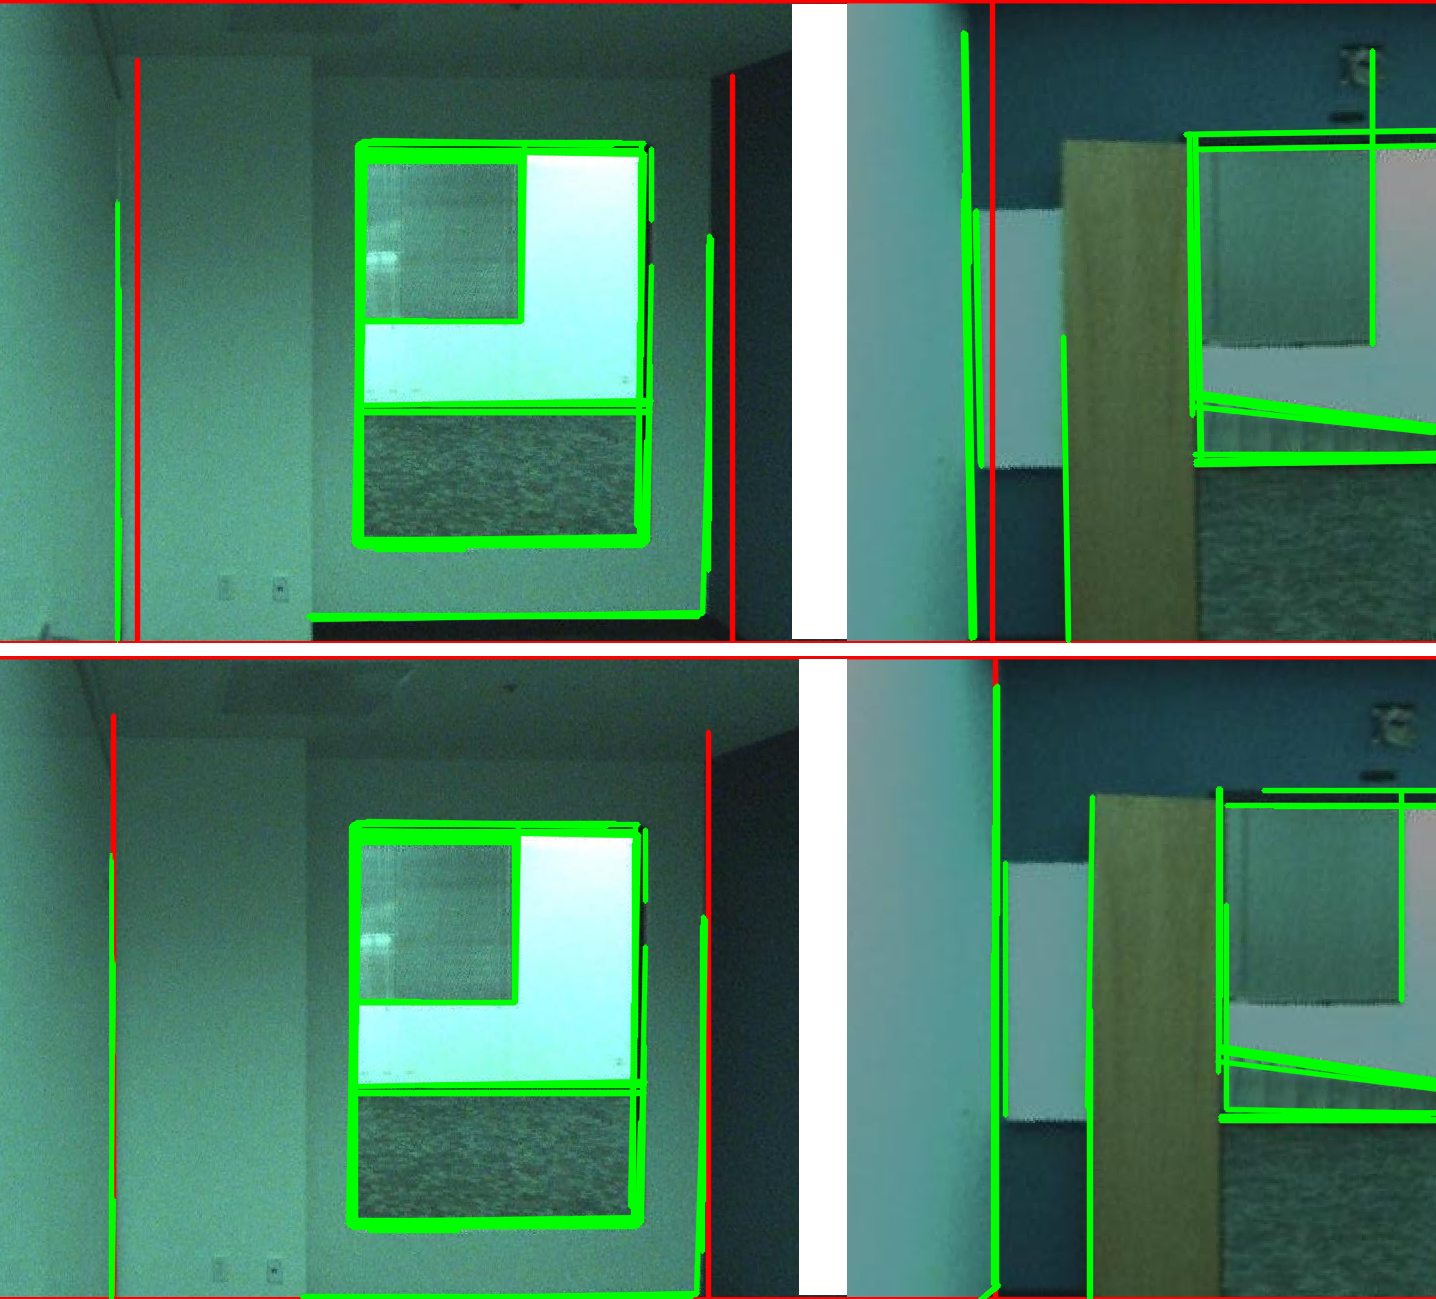
\includegraphics[height=3in,
    width=4in]{bothunalignedaligned.png}}
  \caption{(a) Lines detected in image projections via Hough
    transform.  (b) In this example, we project two images at once for
    the sake of demonstration. Red line segments represent where
    surfaces intersect, and green line segments are line segments
    detected in the image. Above are the original projections using
    input camera poses, and below are the projections after rotation
    and translation for alignment.}
  \label{fig:geometryAlignment}
\end{figure}


Furthermore, at this point in time, image occlusions have not been
accounted for. As a result, some image projections contain texture
that should project to an adjacent surface, sometimes with a visible
linear boundary where the two surfaces meet. If this linear boundary
can be detected by Hough transform, the image is rotated and shifted
in 2D such that the visual boundary between two surfaces in an image
projection matches the physical boundary in our digital model. An
example of such an adjustment is in Figure
\ref{fig:geometryAlignment}(b) and \ref{fig:geometryAlignment}(c).




To perform these alignments, we use a RANSAC \cite{fischler1981random}
framework to determine an optimal rotation angle between lines in our
image and lines in our geometry. RANSAC allows us to ignore erroneous
lines in our image, such as the slanted lines corresponding to the
ladder in Figure \ref{fig:geometryAlignment}(a). Once this rotation is
discovered and applied, we gather all pairs of image line segments and
geometry line segments with less than $0.1^\circ$ difference in
orientation and less than 250 mm distance at their furthest points. If
2 or more pairs exist, we select the 2 that contain the longest
noncollinear image-based line segments, and perform the corresponding
fixed translation to match them. If we only have 1 pair, we perform
the minimal shift to match the lines of that pair, and make note of
their orientation, for usage in Section
\ref{sec:robustSIFTFeatureMatching}.


\subsection{Image Occlusion}
\label{sec:imageOcclusion}
Now that images have been aligned to geometry where possible, we
perform a simple recursive occlusion procedure on each image. This is
done by performing the intersection tests in Section
\ref{sec:simpleTextureMapping} in a regularly spaced grid. Where four
corners of a rectangular region are occluded, texture is
removed. Where no corners are occluded, the recursion stops. Where
there is a mixture of both, the rectangular region is subdivided into
four, and the same process is performed on each. By performing Section
\ref{sec:geometryAlignment}'s alignment procedure before occlusion,
texture belonging to other surfaces is accurately removed, which is
necessary for the next section.

\subsection{2D Feature Alignment}
\label{sec:robustSIFTFeatureMatching}
Our next step is to align images by searching for corresponding points
between all pairs of overlapping images. We use feature alignment
rather than pixel or intensity-based alignment due to the differences
in lighting as well as possible occlusion among our images, both of
which feature alignment is less sensitive to \cite{lowe1999object,
  mikolajczyk2005performance, szeliski2006image}.  We use SiftGPU
\cite{siftgpu} for its high performance on both feature detection as
well as pairwise matching. These matches determine $dx$ and $dy$
distances between each pair of features for two image projections,
though these distances may not always be the same for different
features. Since indoor environments often contain repetitive features
such as floor tiles or doors, we need to ensure that SIFT-based
distances are reliable. First, we only perform alignment on parts of
images that overlap given the original noisy poses. Second, we discard
feature matches that correspond to an image distance greater than 200
mm from what the noisy poses estimate. In order to utilize the
remaining feature matches robustly, RANSAC \cite{fischler1981random}
is again used to estimate the optimal $dx_{i,j}$ and $dy_{i,j}$
distances between two images $i$ and $j$. We use a 5 mm threshold for
RANSAC, so that SIFT matches are labeled as outliers if their distance
is not within 5 mm of the sampled average distance.


We now use the $dx_{i,j}$ and $dy_{i,j}$ distances between each pair
of images, as well as our previous geometry alignment results to refine their positions using weighted linear least
squares. The variables we wish to solve for are the $x_i$ and $y_i$
positions of our images, while our equations are the SIFT-based
distances between pairs of images, images fixed to geometry with 0 or
1 degrees of freedom, and the original camera poses. An example setup for
solving our weighted linear least squares problem $\textrm{min}_{\vec{\beta}} ||W^\frac{1}{2}(A \vec{\beta} -
\vec{\gamma})||_2^2 $ with 3 images is shown below.


\[
A =
\begin{pmatrix}
  -1 & 1 & 0 & 0 & 0 & 0\\
  0 & 0 & 0 & -1 & 1 & 0\\
  0 & -1 & 1 & 0 & 0 & 0\\
  0 & 0 & 0 & 0 & -1 & 1\\
  0 & -m_2 & 0 & 0 & 1 & 0\\
  1 & 0 & 0 & 0 & 0 & 0\\
  0 & 0 & 0 & 1 & 0 & 0\\
  1 & 0 & 0 & 0 & 0 & 0\\
  0 & 0 & 0 & 1 & 0 & 0\\

\end{pmatrix}\quad
\vec{\beta} =
\begin{pmatrix}
  x_1, \\ x_2, \\ x_3, \\ y_1, \\ y_2, \\ y_3
\end{pmatrix}
\vec{\gamma} =
\begin{pmatrix}
  dx_{1,2}, \\ dy_{1,2}, \\ dx_{2,3}, \\ dy_{2,3}, \\ -m_2gx_2 + gy_2, 
  \\ gx_1, \\ gy_1, \\ tx_1, \\ ty_1
  
\end{pmatrix}
\vec{W} = 
\begin{pmatrix}
  1, \\ 1, \\ 1, \\ 1, \\ 1, \\ 1, \\ 1, \\ 0.01, \\ 0.01
\end{pmatrix}
\]


In this scenario, a SIFT-based distance of $dx_{1,2}$, $dy_{1,2}$ was
calculated between images 1 and 2. This corresponds to the first and
second row of $A$, while the third and fourth row of $A$ represent the
same for images 2 and 3. Row 5 corresponds to a constraint of image 2's location to a line of slope $m_2$, passing through point $gx_2$, $gy_2$. 
Row 6 and 7 do stuff and 8 and 9 ensure that we are not rank deficient in case of whatever.

 Rows 5 and 6 of $A$ correspond to a fixed
location of $tx_1$, $ty_1$ for image 1, while Row 7 corresponds to a
constraint to a line of slope $m$, with current location $tx_2$,
$ty_2$, both possible results of the geometry alignment procedure in
Section \ref{sec:geometryAlignment}. If we do not have enough SIFT
matches, or lack images matched to geometry, our matrix becomes
rank-deficient and our problem cannot be solved. As a result, we add
rows for each image corresponding to the original noisy image
locations, and downweight them heavily, e.g. with a weight of 0.01
versus 1.

Because our problem is linear, it is easily and quickly solved, and
after applying the resulting shifts, our images overlap and match each
other with far greater accuracy. Applying the simple mapping scheme in
Section \ref{sec:tileBasedMapping} to the same wall used in that
section results in Figure \ref{fig:compareAll}(b), which has far fewer
discontinuities, though errors due to lighting differences and
parallax effects are still visible.

\section{Image Compositing}
\label{sec:imageCompositing}
In this section, we revisit the tile-based texturing approach from
Section \ref{sec:simpleTextureMapping}, with an added caching
mechanism to reduce image boundaries. This method works well given all
manner of camera poses and surfaces, but for optimal cases where we
have large sections of usable texture from images, we propose a
superior method that further reduces image boundaries.

\subsection{Tile-Mapping with Caching}
\label{sec:mappingWithCaching}
From Section \ref{sec:tileBasedMapping}, we saw that discontinuities
occur where adjacent tiles are textured by different images. Though
Section \ref{sec:2dAlignment}'s image alignment removes many such
discontinuities, there are still cases where seams are visible due to
imprecise matching or other factors such as model-based errors. To
reduce the cases where this happens, it makes sense to take into
account image selections made by neighboring tiles while texture
mapping a given tile. By using the same image across tile boundaries,
we can eliminate a discontinuity altogether. If this is not possible
because a tile is not visible in images used by neighboring tiles,
using similar images across tile boundaries also leads to less
noticeable discontinuities.

Essentially a caching mechanism, we select the best image for a tile
$t$ by searching through two subsets of images for a viable candidate,
before searching through the entire set of valid images. The first
subset of images is the images selected by adjacent tiles that have
already been textured. We must first check which of these images can
map to $t$, and then of those, we make a choice according to the
scoring function in Figure \ref{fig:scoringFunction}. Before reusing
this image, we ensure it meets the criteria $\alpha < 45^\circ$, in
order to ensure a high resolution projection, with $\alpha$ as the
camera angle as shown in Figure \ref{fig:scoringFunction}.

If no satisfactory image is found in the first subset, we check a
second subset of images, consisting of those taken near the ones in
the first subset, both spatially and temporally. These images are not
the same as the ones used for neighboring tiles, but are taken at a
similar location and time, suggesting that their localization and
projection are quite similar, and thus likely matched more cleanly. If
no viable image is found according to the same criteria as before, we
search the entire set of candidate images, selecting based on the same
scoring function from Figure \ref{fig:scoringFunction}.

The result of this caching approach is shown in Figure
\ref{fig:compareAll}(c), where seams are now reduced as compared to
Figure \ref{fig:compareAll}(b). However, some discontinuities are
still present, as visible in the posters on the wall with breaks in
their borders.

\begin{figure}
  \centering
  \subfloat[][]{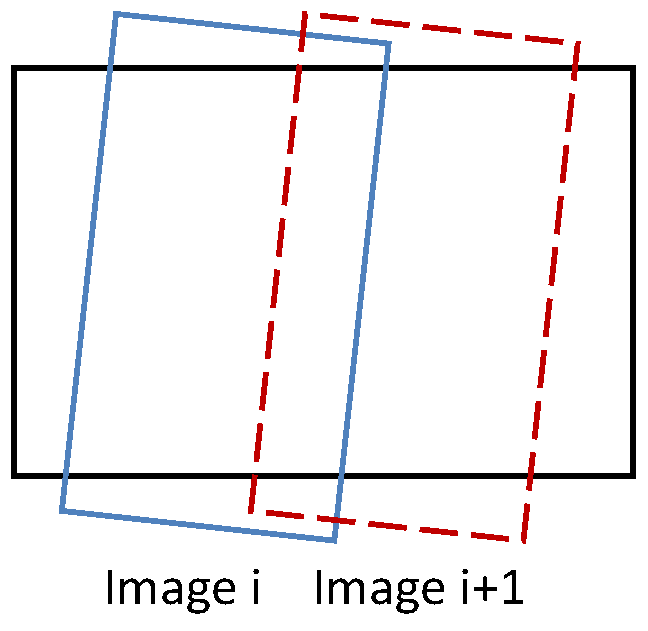
\includegraphics[width=1in]{projectionWall.pdf}}
  \centering
  \subfloat[][]{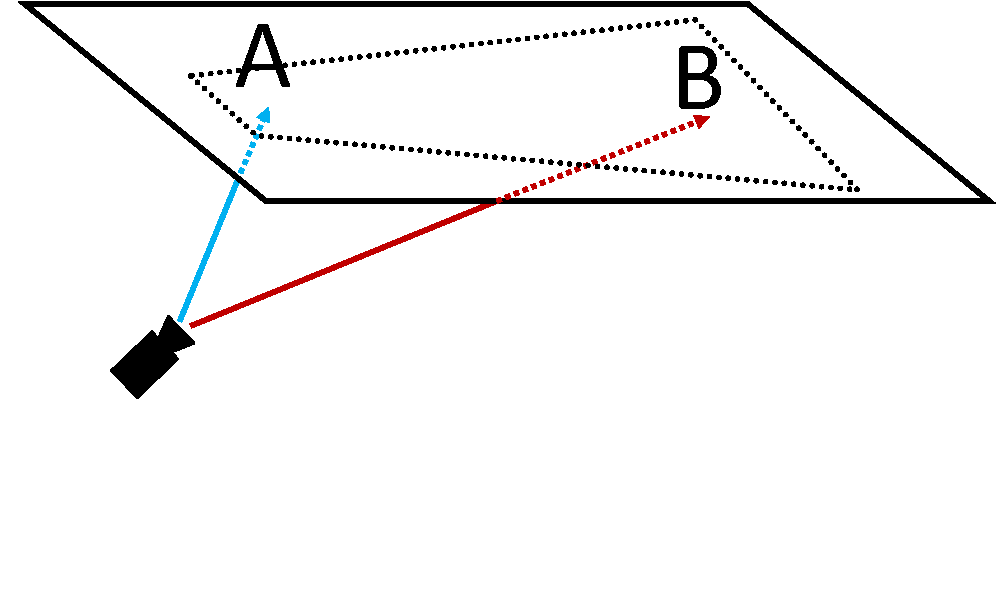
\includegraphics[width=1.1in]{projectionCeiling.pdf}}
  \centering
  \subfloat[][]{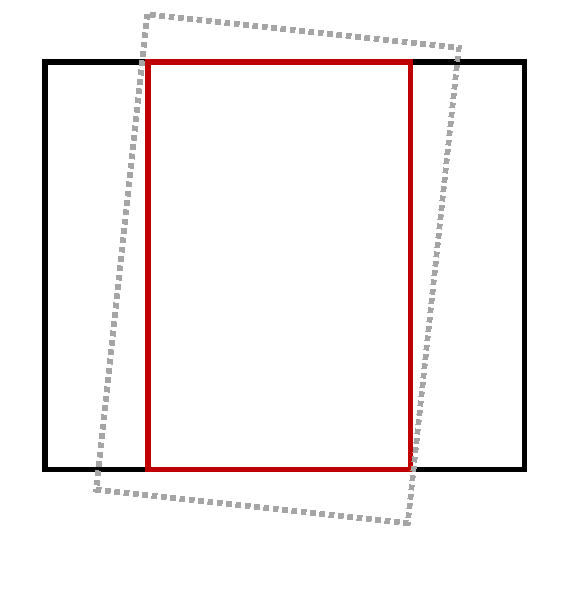
\includegraphics[width=0.9in]{projectionWallCrop.pdf}}
  \caption{(a) Images for vertical planes are tilted, but their camera
    axes are more or less normal to their respective planes. (b)
    Camera axes for ceiling images are at large angles with respect to
    plane normals. (c) Wall images are cropped to be rectangular.}
  \label{fig:projectionAngles}
\end{figure}


As mentioned earlier, our data comes from a mobile backpack
system. Human operators can not carry the backpack in a perfectly
upright position and are bent forwards at 15 to 20 degrees with
respect to the vertical direction. As a result, cameras facing
sideways are head on with respect to vertical walls, while cameras
oriented towards the top or bottom of the backpack are at an angle
with respect to horizontal floors and ceilings. This is depicted in
Figures \ref{fig:projectionAngles}(a) and
\ref{fig:projectionAngles}(b). These oblique camera angles for
horizontal surfaces translate into textures that span large areas once
projected, as shown in Figure \ref{fig:projectionAngles}(b). Using the
tile-based texture mapping criteria from Figure
\ref{fig:scoringFunction}, such projections have highly varying scores
depending on the location of a tile on the plane. Thus, the tiling
approach in this section is a good choice for texturing floors and
ceilings, as it uses the parts of image projections that maximize
resolution and accuracy for their respective plane locations,
e.g. areas near point A and not near point B, in Figure
\ref{fig:projectionAngles}(b).


\subsection{Shortest Path Texturing}
\label{sec:shortestPath}
For vertical walls, most images are taken from close distances and
head-on angles, resulting in high resolution fronto-parallel
projections. As a result, for each tile on a wall plane, the scoring
function of Figure \ref{fig:scoringFunction} is relatively flat with
respect to candidate images, as they are all more or less head
on. Thus, the scoring function is less significant for walls, and it
is conceivable to use a different texturing strategy to directly
minimize visible seams when texturing them. This is done by choosing
the smallest possible set of images that (a) covers the entire plane
and (b) minimizes the visibility of borders between them. A
straightforward cost function that accomplishes the latter is the sum
of squared differences (SSD) of pixels in overlapping regions between
all pairs of images. Minimizing this cost function encourages image
boundaries to occur either in featureless areas, such as bare walls,
or in areas where images match extremely well.

The first step in this procedure is to obtain a list of images useful
for texturing the wall. A simple way to do this is to use the images
selected by the tiling process in Section
\ref{sec:tileBasedMapping}. Such a list of images is guaranteed to
cover the entire wall, and consists of desired camera poses overall.

In the general case, our problem can be defined as minimally covering
a polygon i.e. the planar surface, using other polygons of arbitrary
geometry i.e. image projections, with the added constraint of
minimizing the cost function between chosen images. Given that
wall-texture candidate images are taken from more or less head-on
angles, and knowing that only minor rotations are made in Section
\ref{sec:2dAlignment}, we can crop our image projections to be
rectangular with minimal texture loss. Furthermore, because our
fisheye camera lenses have full floor-to-ceiling coverage of nearly
all walls, and our backpack operator logically only moves
horizontally, we only need to ensure lateral coverage of our wall
planes. We can thus construct a Directed Acyclic Graph (DAG) from the
images, with edge costs defined by the SSD cost function, and solve a
simple shortest path problem to find an optimal subset of images with
regard to the SSD cost function \cite{dijkstra}.

\begin{figure}
  \centering
  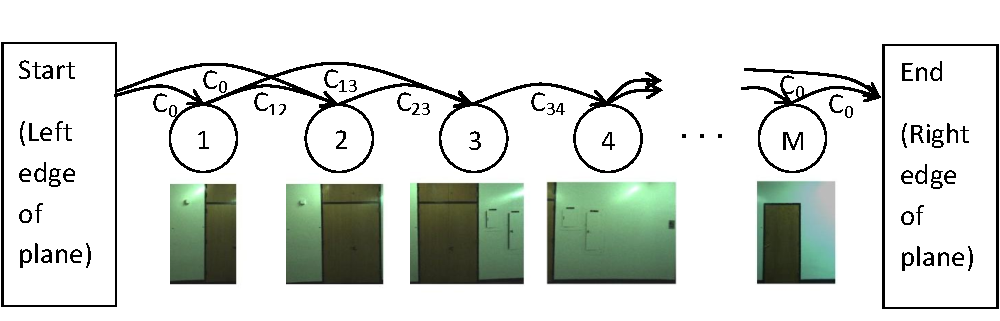
\includegraphics[width=5in]{dagCreation.pdf}
  \caption{DAG construction for the image selection process. \\}
  \label{fig:dagCreation}
\end{figure}

Figure \ref{fig:dagCreation} demonstrates the construction of a DAG
from overlapping images of a hallway wall. Images are sorted by
horizontal location left to right, and become nodes in a
graph. Directed edges are placed in the graph from left to right
between overlapping images. The weights of these edges are determined
by the SSD cost function. Next, we add two artificial nodes, one start
node representing the left border of the plane, and one end node
representing the right border of the plane. The left(right) artificial
node has directed edges with equal and arbitrary cost $C_0$ to(from)
all images that meet the left(right) border of the plane. We now solve
the shortest path problem from the start node to the end node. This
results in a set of images completely covering the plane horizontally,
while minimizing the cost of seams between images.

In very rare cases where the vertical dimension of the plane is not
entirely covered by one or more chosen images, we are left with holes
where no images are selected to texture. Since these holes are rare,
and generally fairly small, we use a greedy approach, repeatedly
filling the hole with images that result in the lowest SSD costs in a
blending region around the hole, as discussed in Section
\ref{sec:blending}. This method is not as optimal as a true
2D-coverage solution would be, but it is a fast approximation, and
adequately handles the few holes we encounter.

With this completed, we have now mapped every location on the plane to
at least one image, and have minimized the number of images, as well
as the discontinuities at their borders. As seen in Figure
\ref{fig:compareAll}(d), this shortest path method has fewer visible
discontinuities than Figure \ref{fig:compareAll}(c) corresponding to
the tile caching approach\footnote{In Figure \ref{fig:compareAll}(d),
  we arbitrarily chose one image for texturing where images overlap,
  as blending will be discussed in section \ref{sec:blending}.}. This
is especially evident when comparing the posters in the images. This
shortest path approach approach directly reduces the cost of each
image boundary, while the tile caching method uses a scoring function
that only approximates this effect. Furthermore, this approach
guarantees the best selection of images to minimize seams, while the
sequential tile caching method may select images early on that turn
out to be poor choices once subsequent tiles have been processed. This
shortest path approach is also far less intensive in terms of memory
usage and runtime, both during texture generation and rendering, as it
does not require discretizing planes or images.

When texturing an entire 3D planar model, we apply the shortest path
method on walls, due to its superior output when provided with head-on
images. Floors and ceilings however, given their many images taken at
oblique angles, are textured using the tile caching method.


\subsection{Blending}
\label{sec:blending}
We now apply a blending procedure to both texturing methods. Although
the image alignment steps and image selection in both methods attempt
to minimize all mismatches between images, there are occasional
unavoidable discontinuities in the final texture due to different
lighting conditions or inaccuracies in model geometry. These can
however be treated and smoothed over by applying alpha blending over
image seams.  Whether the units we are blending are
rectangularly-cropped images or rectangular tiles, we can apply the
same blending procedure, as long as we have a guaranteed overlap
between units to blend over.

For the tile caching method, we can ensure overlap by texturing a
larger tile than needed for display. For example, for a rendered tile
$l_1 \times l_1$, we can associate it with a texture $(l_1 + l_2)
\times (l_1 + l_2)$ in size.  We have found $l_2 = \frac{l_1}{2}$ to
provide a balance between blending and keeping features unblurred. For
the shortest path method, we have already ensured overlap between
images. To enforce consistent blending however, we add a minimum
required overlap distance of 200 mm while solving the shortest path
problem in Section \ref{sec:shortestPath}. Additionally, if images
overlap in a region greater than the overlap distance, we only apply
blending over an area equal to the overlap distance.

After performing linear alpha blending across overlapping regions, our
texture mapping process is complete. Figures \ref{fig:compareAll}(e)
and \ref{fig:compareAll}(f) show the blended versions of Figures
\ref{fig:compareAll}(c) and \ref{fig:compareAll}(d) respectively. The
remaining images in Figure \ref{fig:compareAll} highlight differences
between the two methods, showing that Figure \ref{fig:compareAll}(f)
has the best visual quality and the best texturing approach among the
textures in Figure \ref{fig:compareAll}.

\section{Results and Conclusions}
\label{sec:resultsAndConclusions}
Examples of ceilings and floors textured with the tile caching
approach, and walls textured with the shortest path approach, are
displayed in Figure \ref{fig:results}. These results are as accurate
and clean as the best results we obtained using the two algorithms
mentioned in Section \ref{sec:existingApproaches}. High resolution
colored texture comparisons, as well as video and interactive
walkthroughs of full models are available at
\footnote{\url{http://www.eecs.berkeley.edu/~pcheng/indoormapping}}.

As mentioned earlier, our approach is quite efficient. The top wall in
Figure \ref{fig:results}(a) was generated with 7543 $\times$ 776
pixels, and spans a 40-meter long wall. Given 41000 input images of
the entire dataset, a 2.8GHz dual-core consumer-grade laptop takes
approximately a minute to pick 36 candidate images, followed by under
a minute to perform both image alignment and the shortest path
texturing method, though over 75\% of that time is spent calculating
SIFT matches within the SiftGPU framework. While not real-time, the
process is capable of generating quick updates after changes in
various parameters or modifications to input data, and if integrated
directly into a modeling system, could provide live visualization as
data is collected. Our full models consist of our input model file,
textures that we generate, and a mapping of image points to model
vertices. The models shown in Figure \ref{fig:results} are roughly 20
MB in size, and are visualized using the OpenSceneGraph toolkit
\cite{openscenegraph}, which allows for export to many common model
formats, as well as efficient visualization, even in web browsers or
mobile devices.

In this paper, we have developed an approach to texture mapping models
with noisy camera localization data. We are able to refine image
locations based on geometry references and feature matching, and
robustly handle outliers. Using the tile-based mapping approach, we
can texture both simple rectangular walls as well as complex floor and
ceiling geometry. We also implemented a shortest path texturing method
that produces seamless textures on planes where multiple head-on
images are available. Both of these approaches are highly modular, and
easily tunable for similar systems across multiple environments.

\subsection{Future Work}
While our method works well on our datasets, it is heavily reliant on
having a large number of input images, and minimal non-2D error. A
technique for resolving camera error in 3D that would mesh well with
our approach is to perform matching between image lines and geometry
in 3D, which can be done reasonably efficiently \cite{linebased,
  rectangularstructures}. Using linear features on top of our SIFT
features is also likely to result in improved matches, as indoor
scenes often have long, unbroken lines spanning multiple images
\cite{linearposeestimation}. Finally, our blending approach is quite
basic, and applying more sophisticated methods of blending as well as
normalization would benefit our final visual quality, and more
robustly handle motion-based or parallax errors.



\begin{figure}
  \centering
  \subfloat[][]{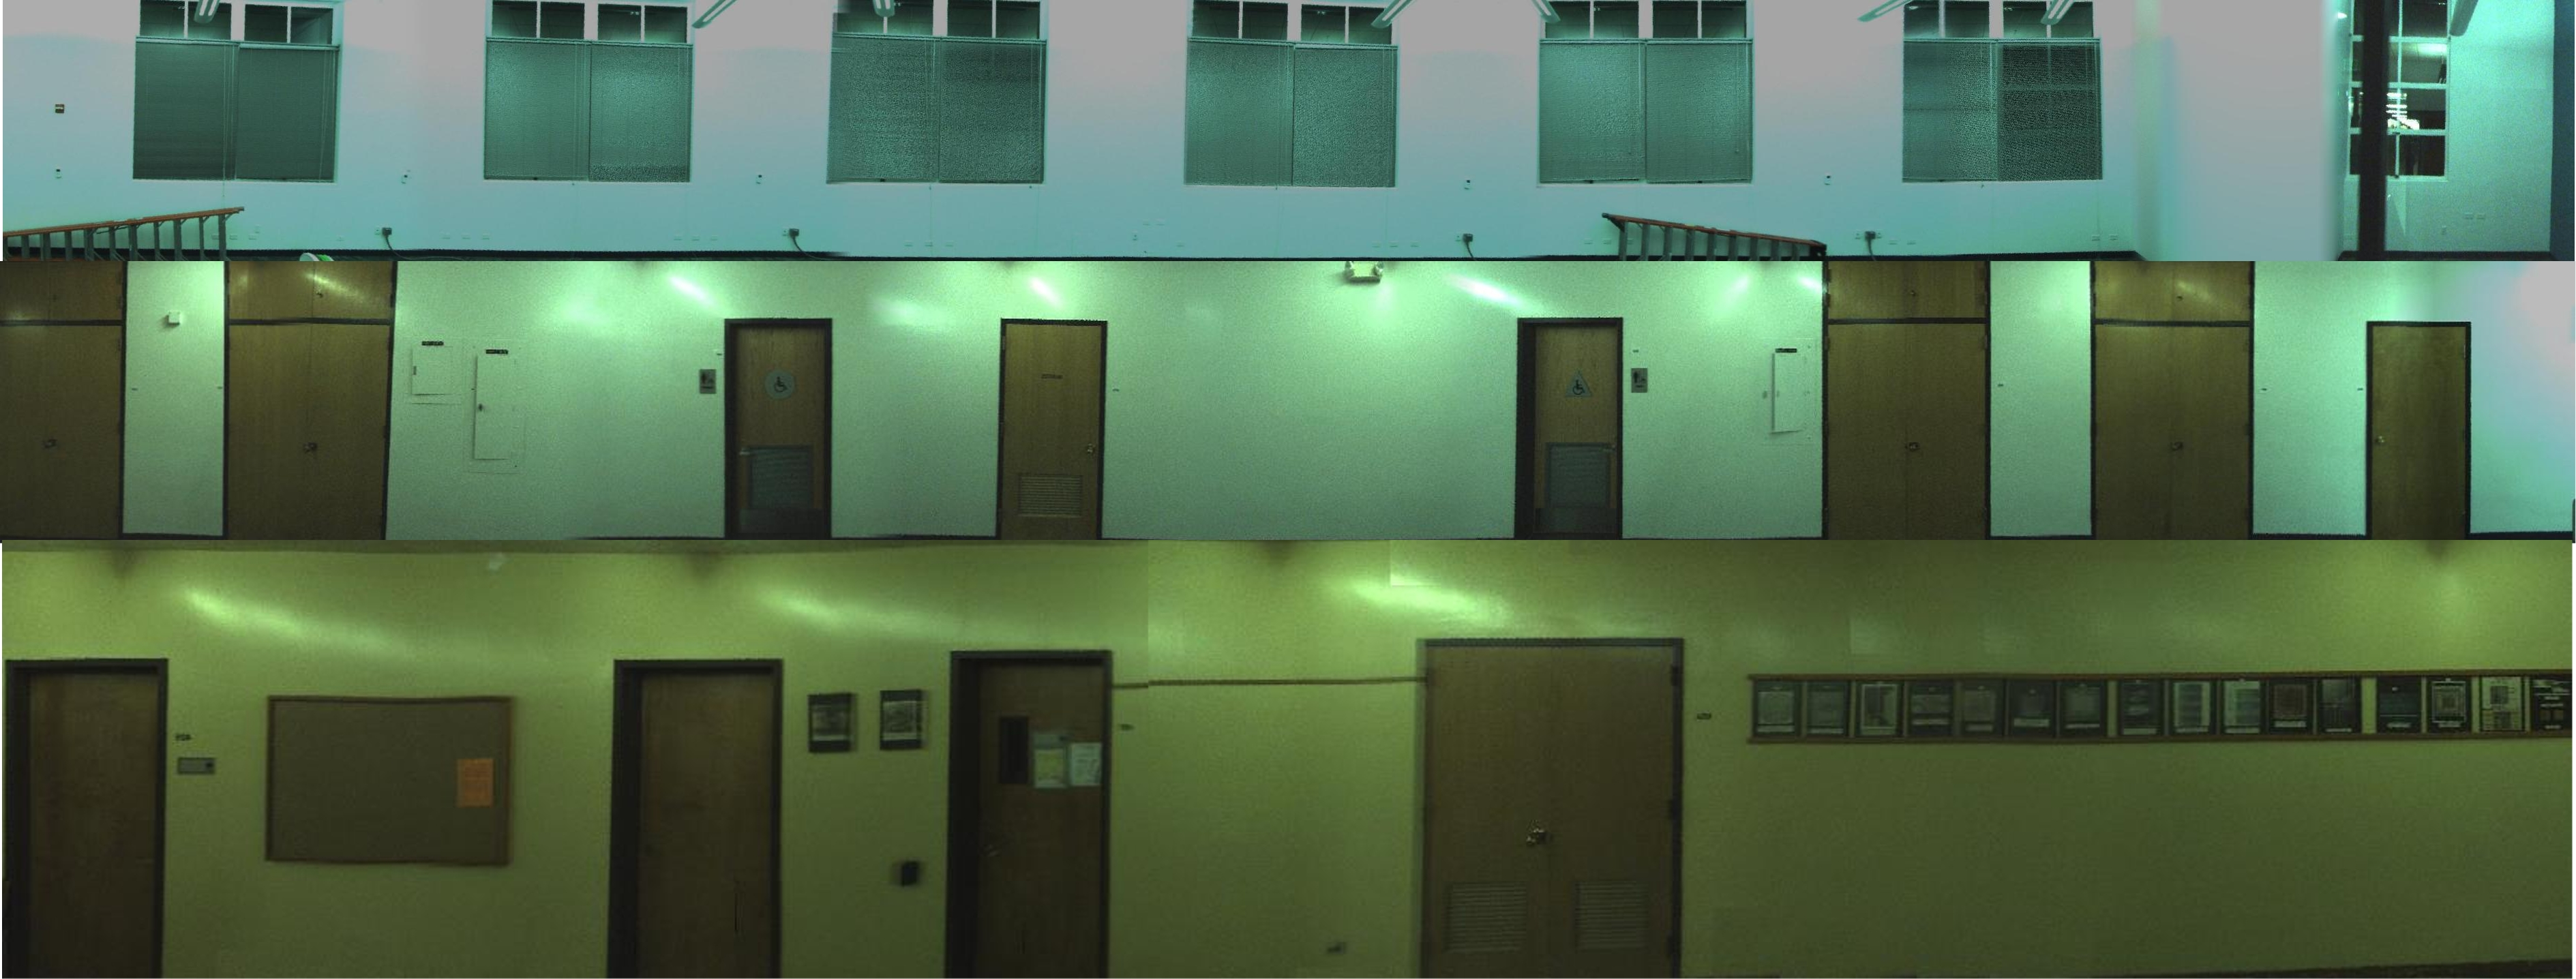
\includegraphics[width=3in]{finalfloors.jpg}} ~~~~~~~~
  \centering
  \subfloat[][]{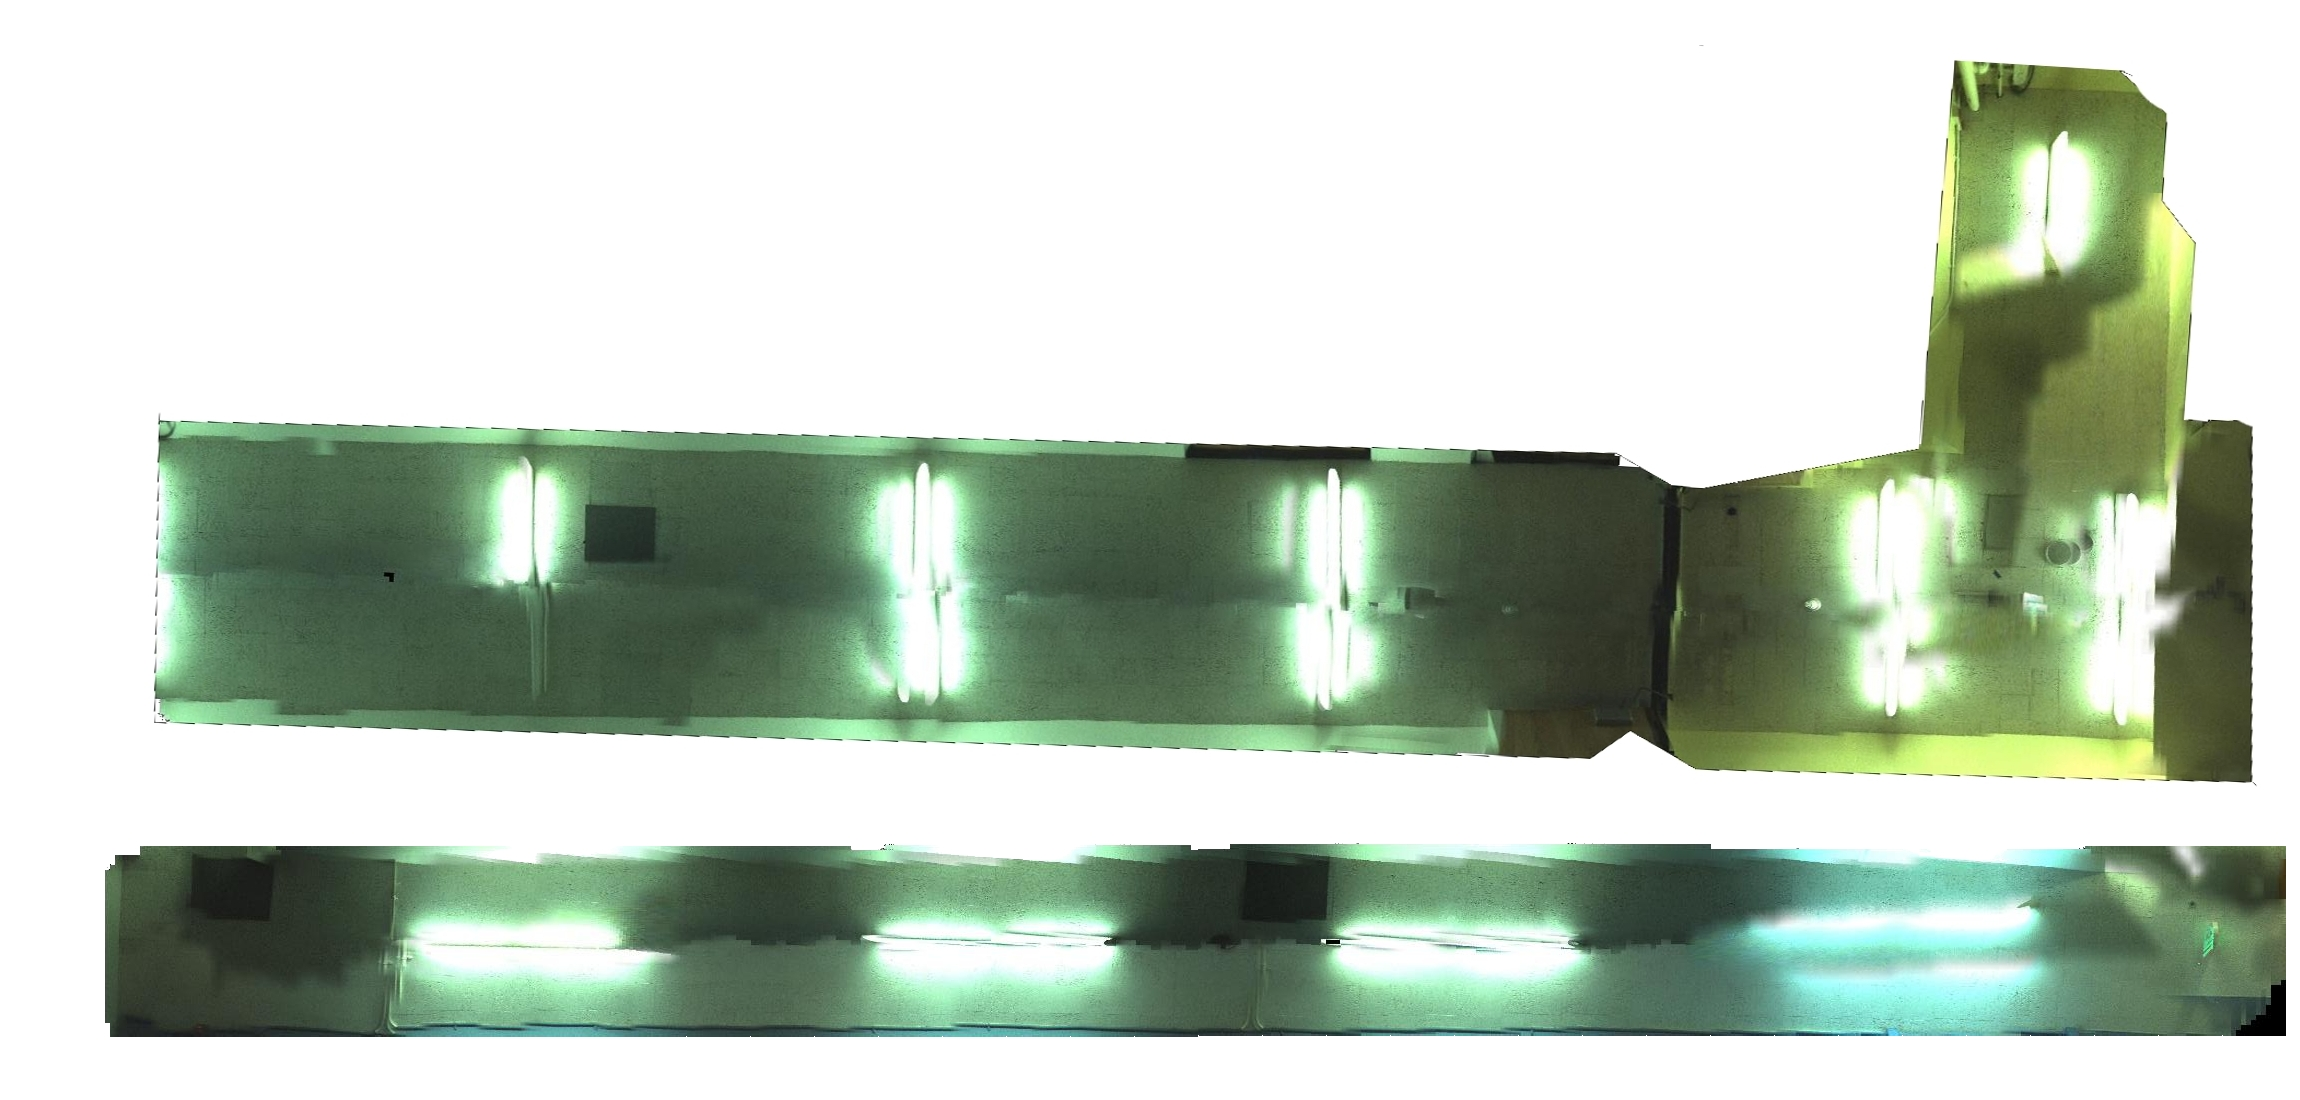
\includegraphics[width=3in]{finalceilings.jpg}}

  \centering \subfloat[][]{
    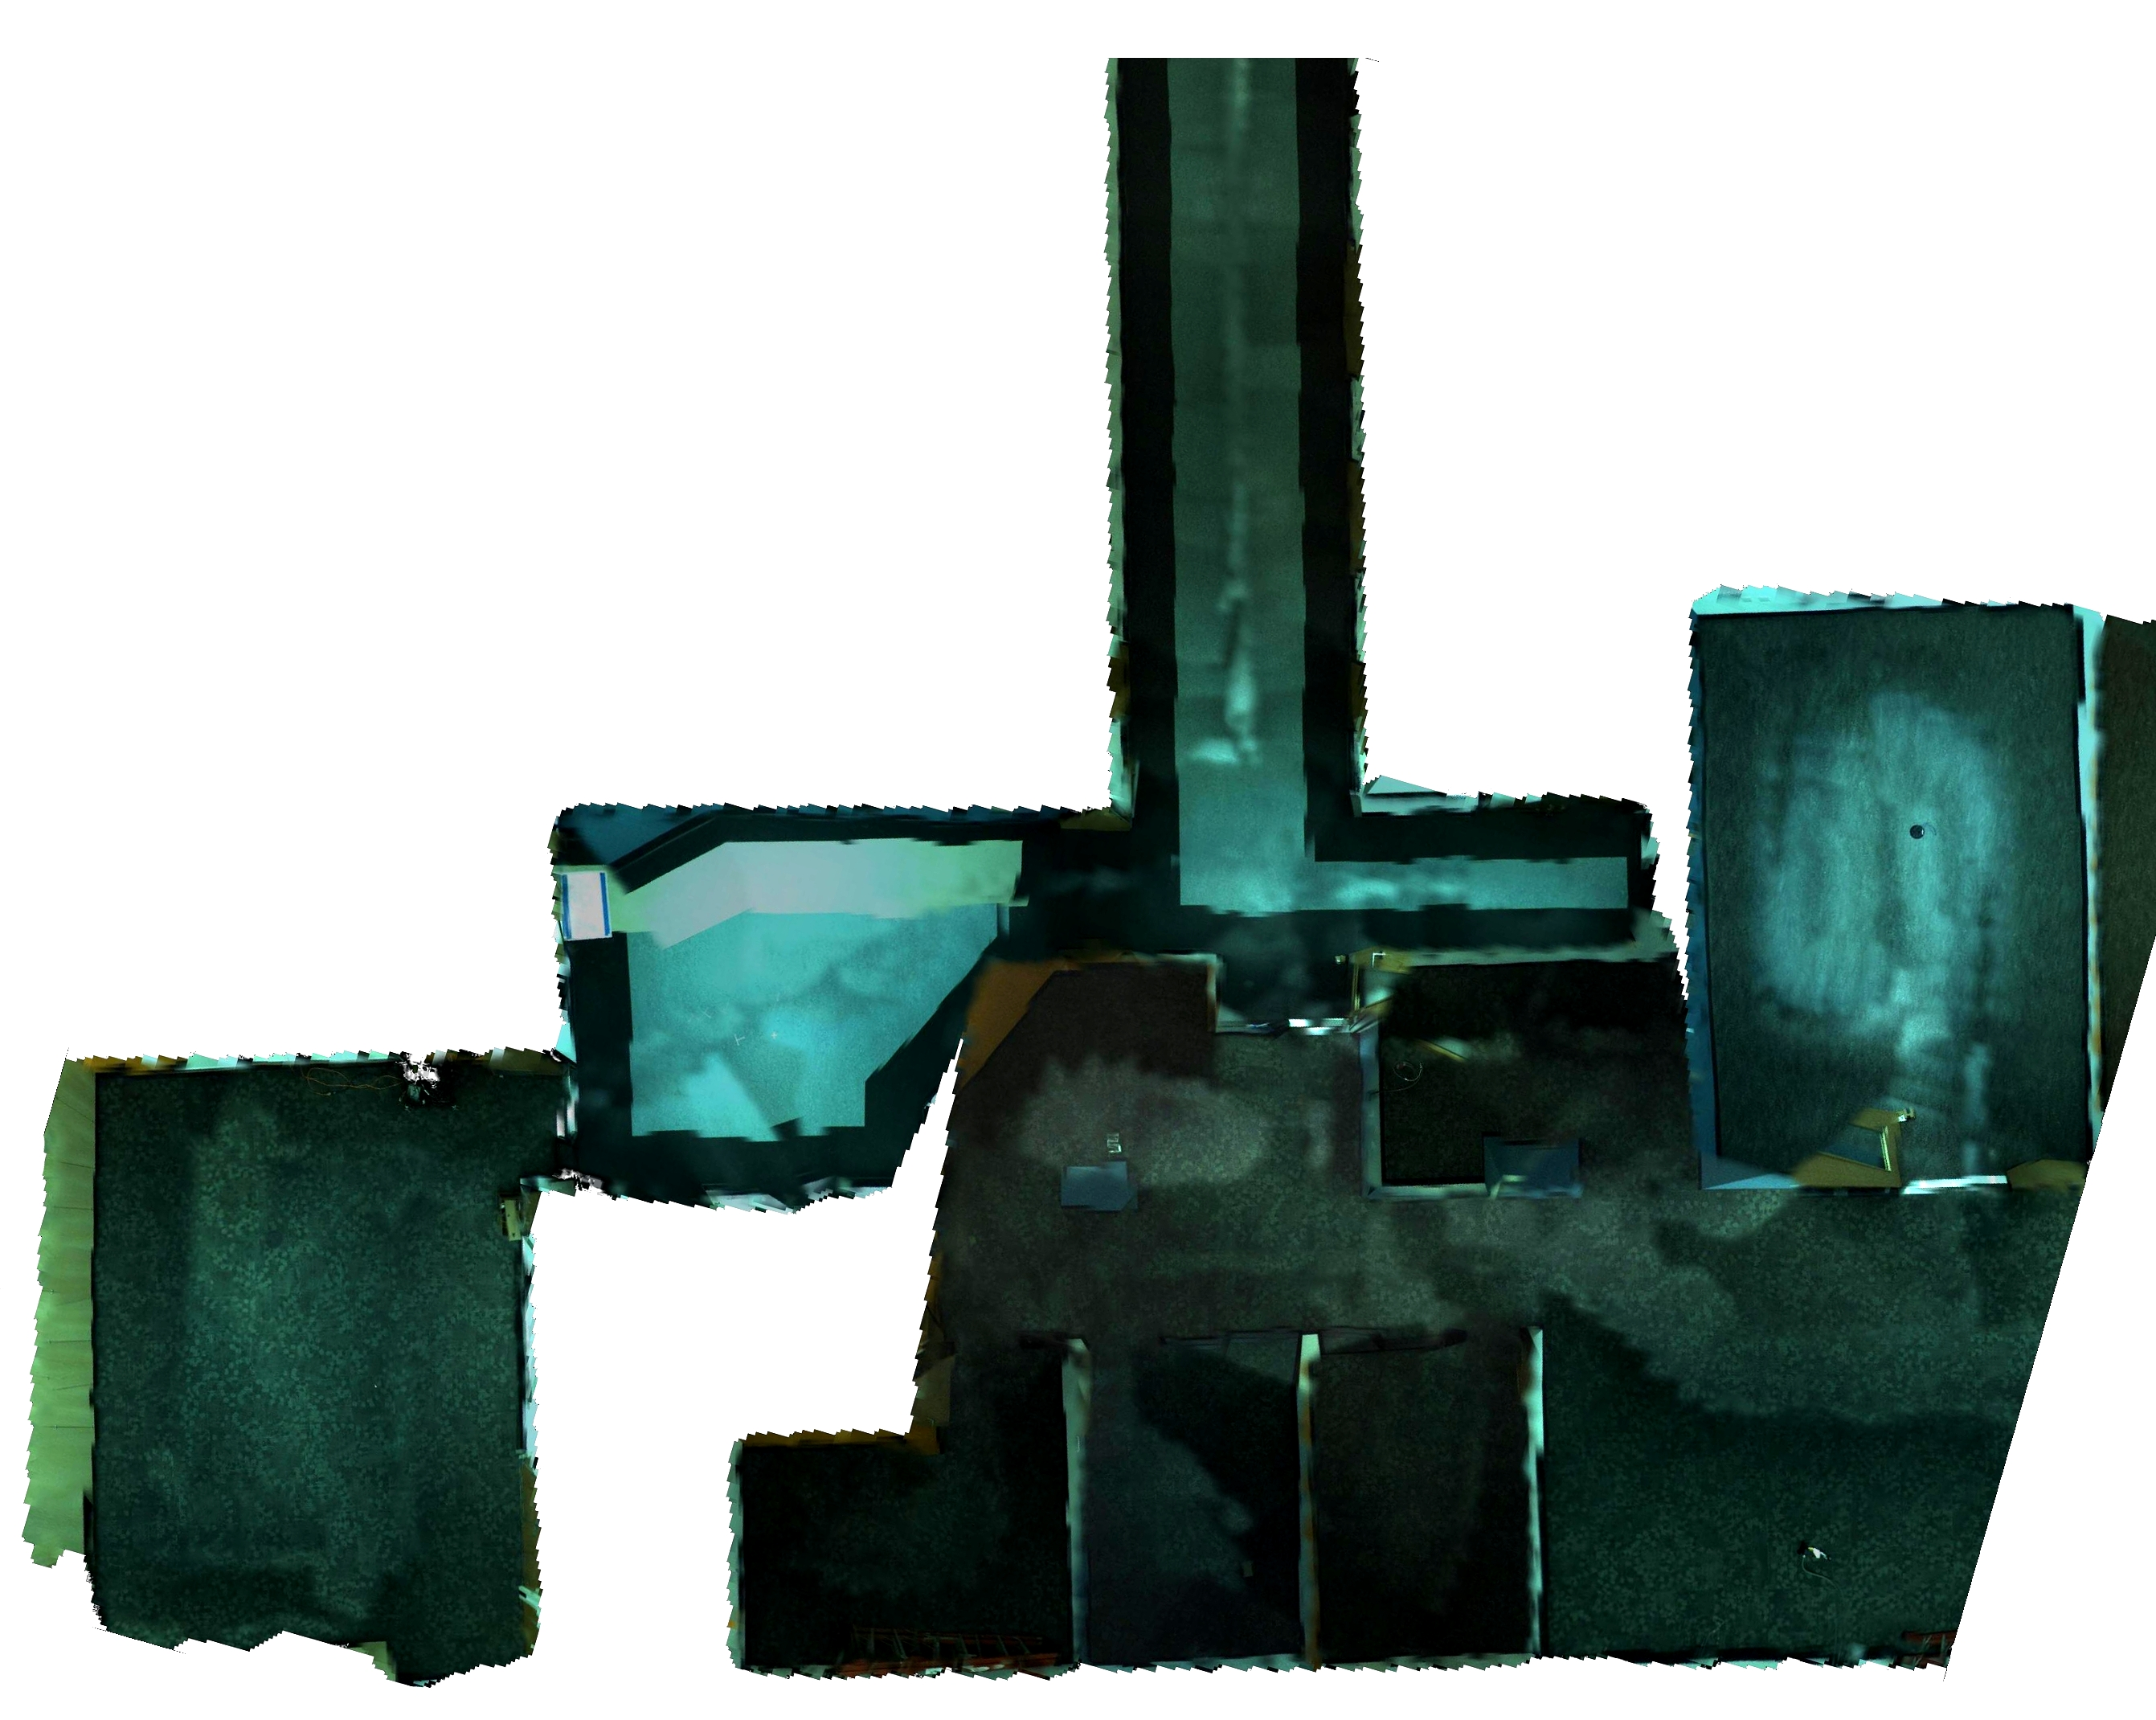
\includegraphics[height=2in, width=3in]{floorcropped.jpg} ~~~~~~~~
    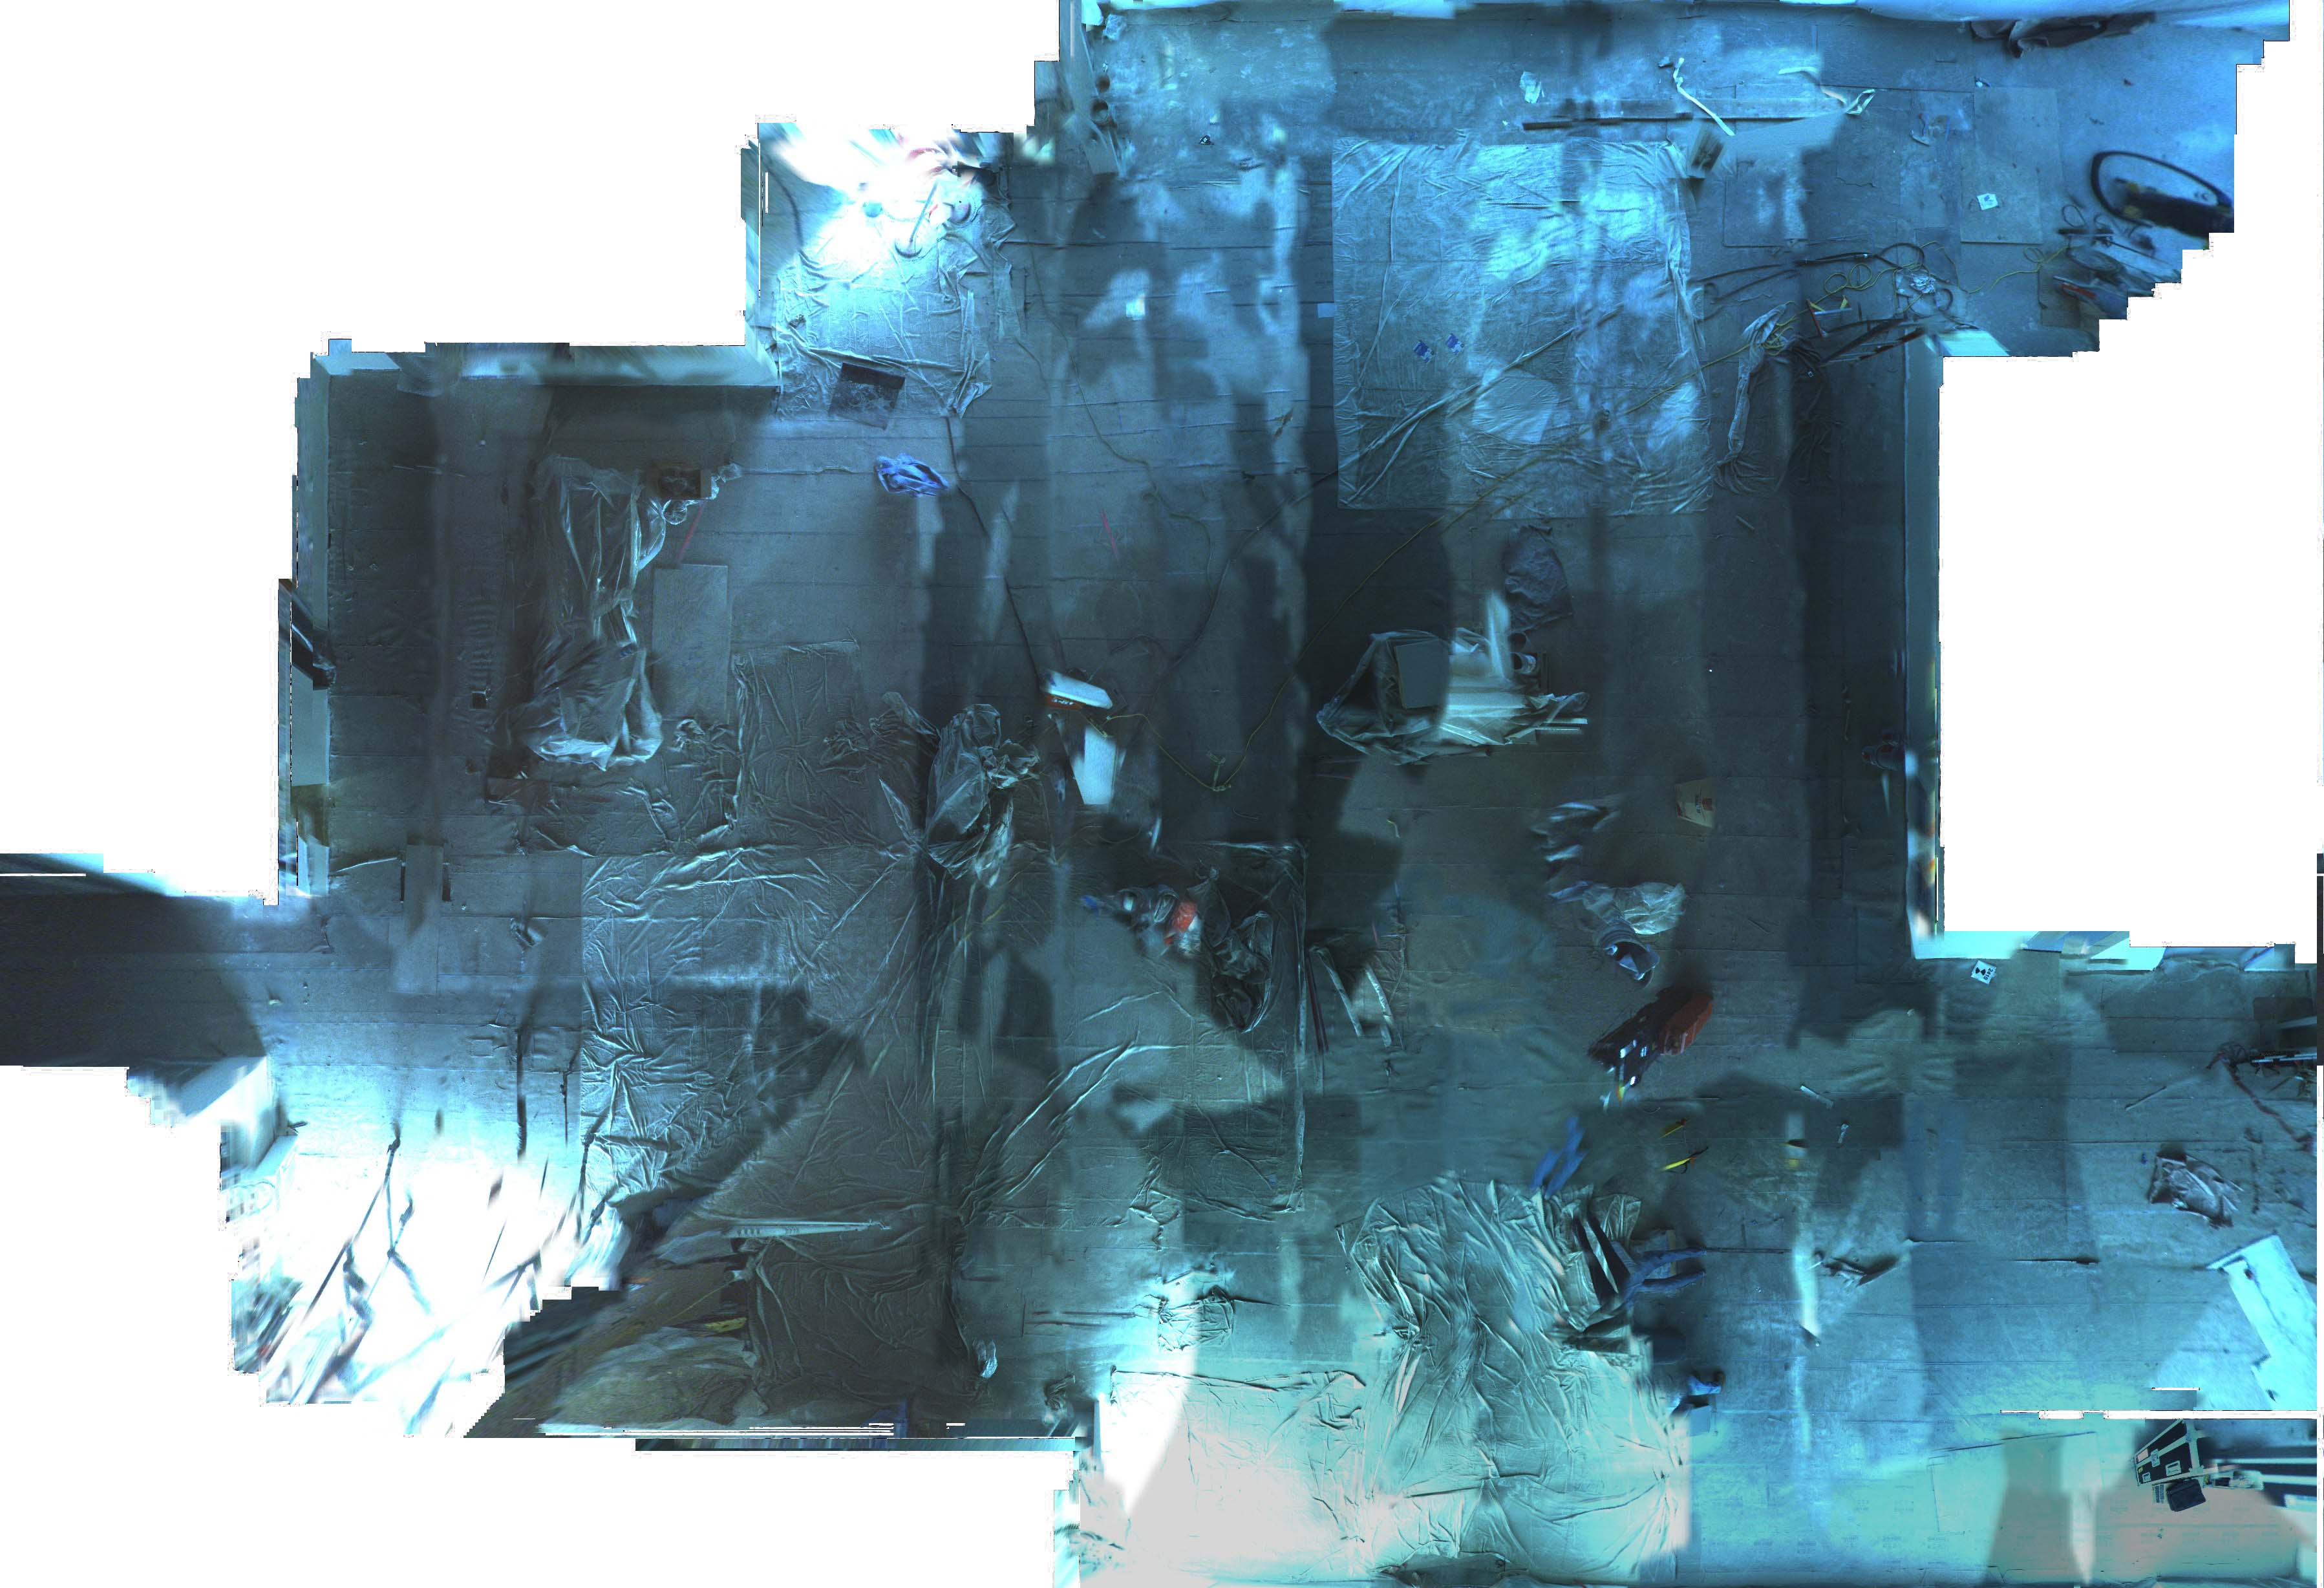
\includegraphics[width=3in]{pier15floor.jpg}
  }

  \centering{
    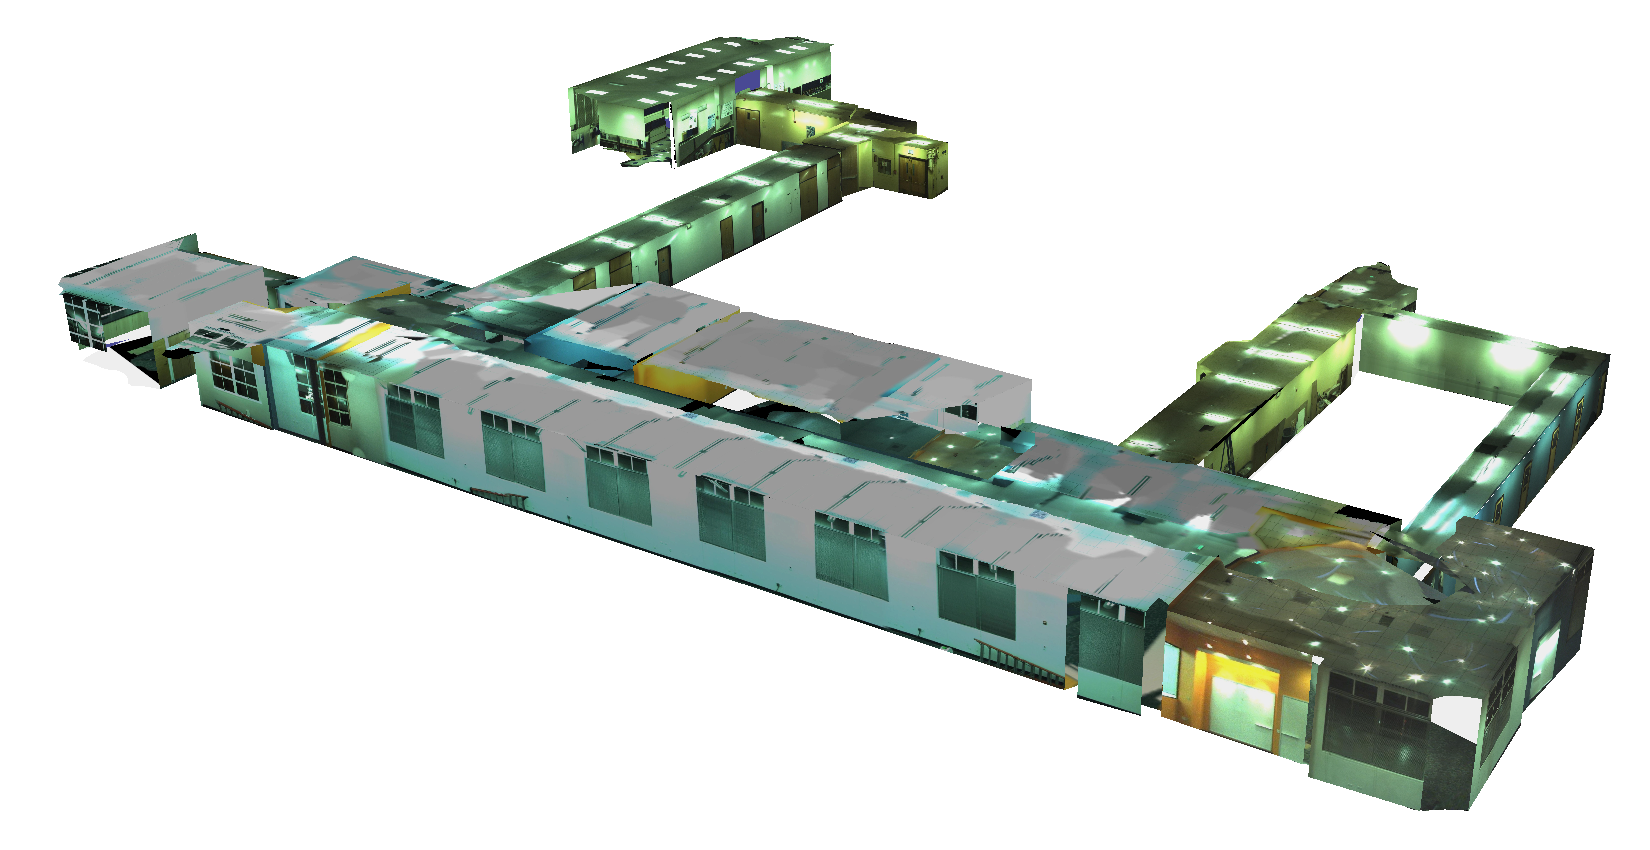
\includegraphics[width=1.9in]{fullmodel.png}
    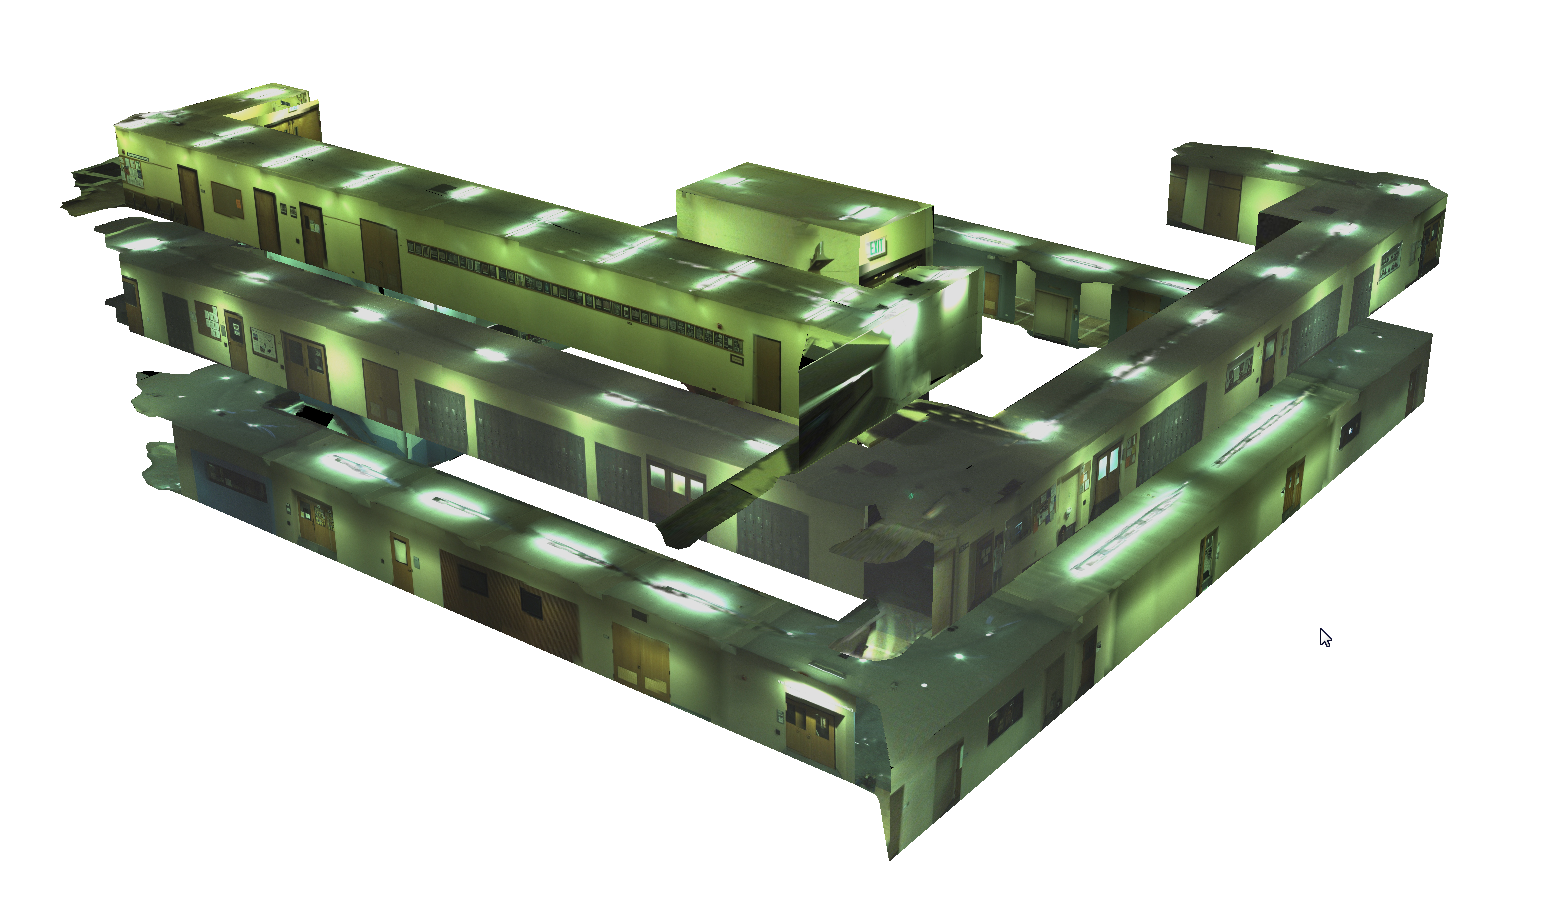
\includegraphics[width=1.9in]{threestoryfull2.png}
    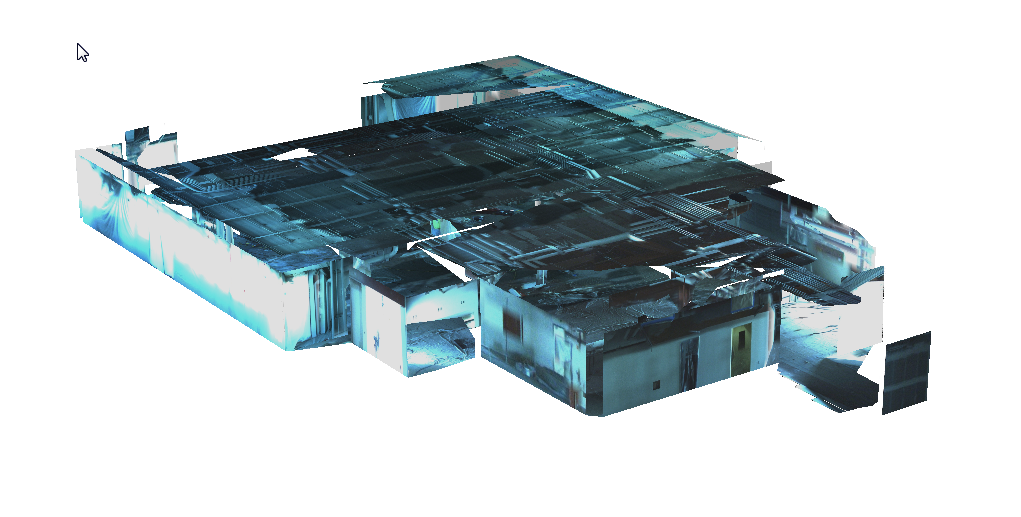
\includegraphics[width=1.9in]{pier15.png} \\
    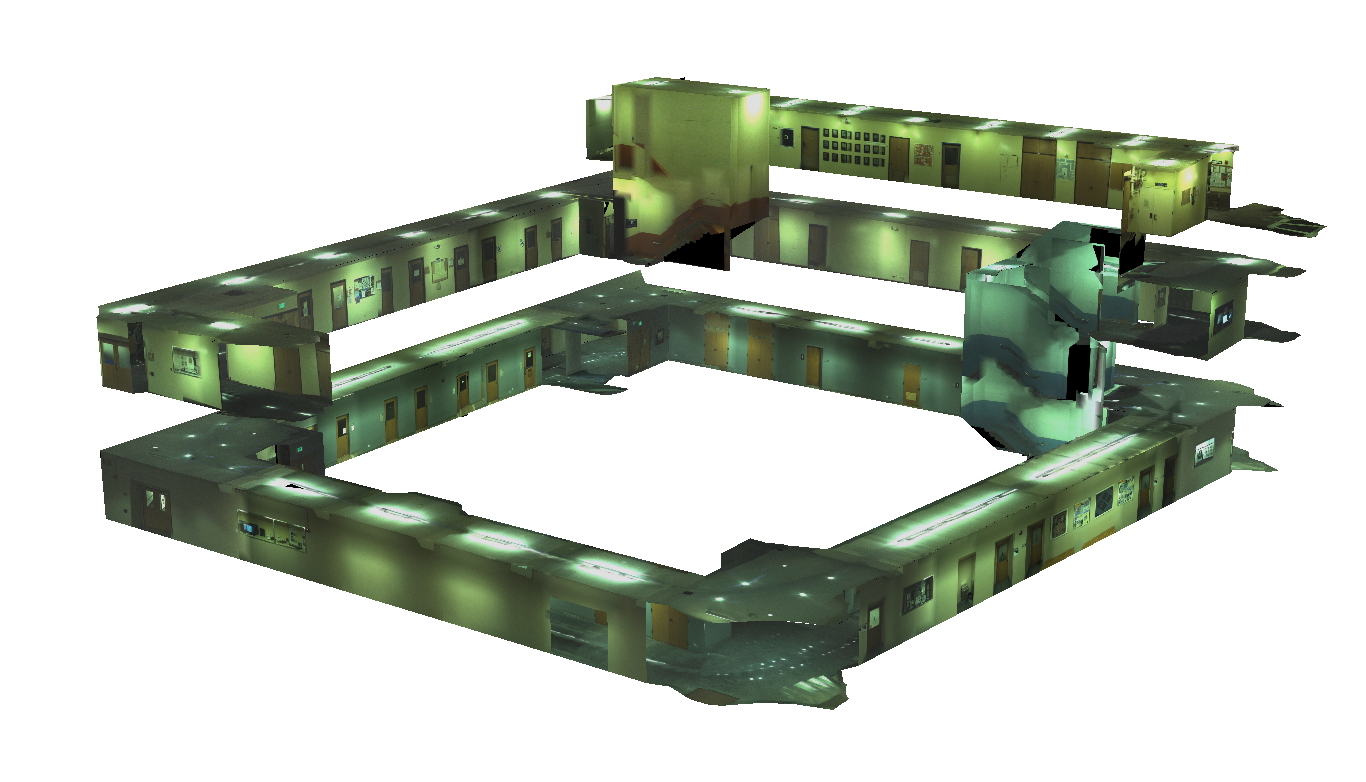
\includegraphics[width=6in]{threestoryfull.png}
  }

  \centering \subfloat[][]{ }
  \caption{Examples of our final texture mapping output for (a) walls,
    (b) ceilings, (c) floors, (d) full models.}
  \label{fig:results}
\end{figure}


%%%%%%%%%%%%%%%%%%%%%%%%%%%%%%%%%%%%%%%%%%%%%%%%%%%%%%%%%%%%%
%%%%% References %%%%%

\bibliography{report} %>>>> bibliography data in report.bib
\bibliographystyle{spiebib} %>>>> makes bibtex use spiebib.bst

\end{document} 
